\chapter{Historical Notifications, Data Analysis and Result Validation} \label{chp:historical-notifications-data-analysis-validation}

This chapter presents the data used in this work, the analysis of the data, and the validation of the results.

\section{Limoeiro do Norte and Alto Santo Cities} \label{sec:real-notifications}

This section presents an analysis of the cases notified in the cities of \textit{Alto Santo} and \textit{Limoeiro do Norte} in the state of Ceará, Brazil. These notifications are from 2015 to 2022 and were obtained through the city health departments through \gls{sinan}~\cite{laguardia:2004}. The data is organized in tables that contain 157 information fields from the medical service sheets. From \textit{Alto Santo} city, we obtained 630 notifications in the data from 2016 to 2022. \textit{Limoeiro do Norte} city has reported 3829 Dengue and 414 Chikungunya cases between 2015 and 2021. The data from both cities gives a total of 4873 cases reported in the \gls{sinan}.

According to \gls{ibge}\footnote{\url{https://www.ibge.gov.br/}}, in the last demographic census conducted in 2022, the \textit{Alto Santo} resident population was 14,155 people. In \textit{Limoeiro}, this value increases to 59,560 residents, more than four times the population of \textit{Alto Santo}. The urban area of \textit{Alto Santo} is only about 2 km$^2$, while \textit{Limoeiro} has almost 15 km$^2$. The city centers extracted from \gls{osm} are presented in Figure~\ref{fig:graph-examples}.

\begin{figure}[h!]
\centering
  \begin{minipage}[c]{.45\textwidth}
    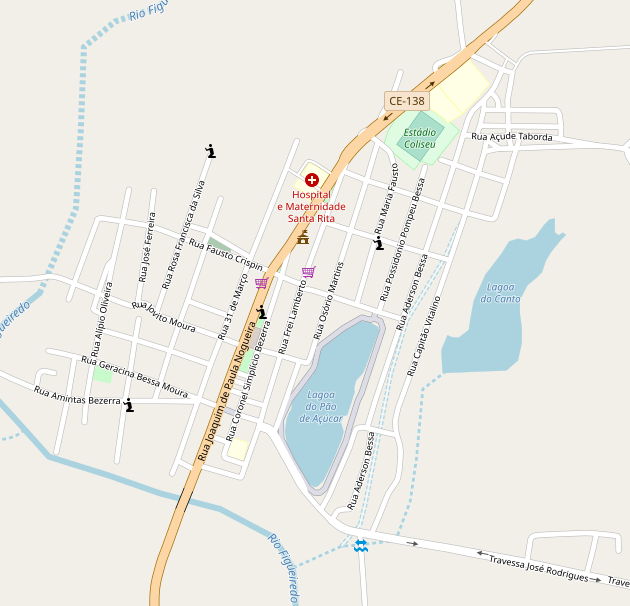
\includegraphics[width=6cm, height=5cm]{images/alto-santo-osm.png}
    \subcaption{Map of Alto Santo downtown.}
  \end{minipage}
  \hfill
  \begin{minipage}[c]{.45\textwidth}
  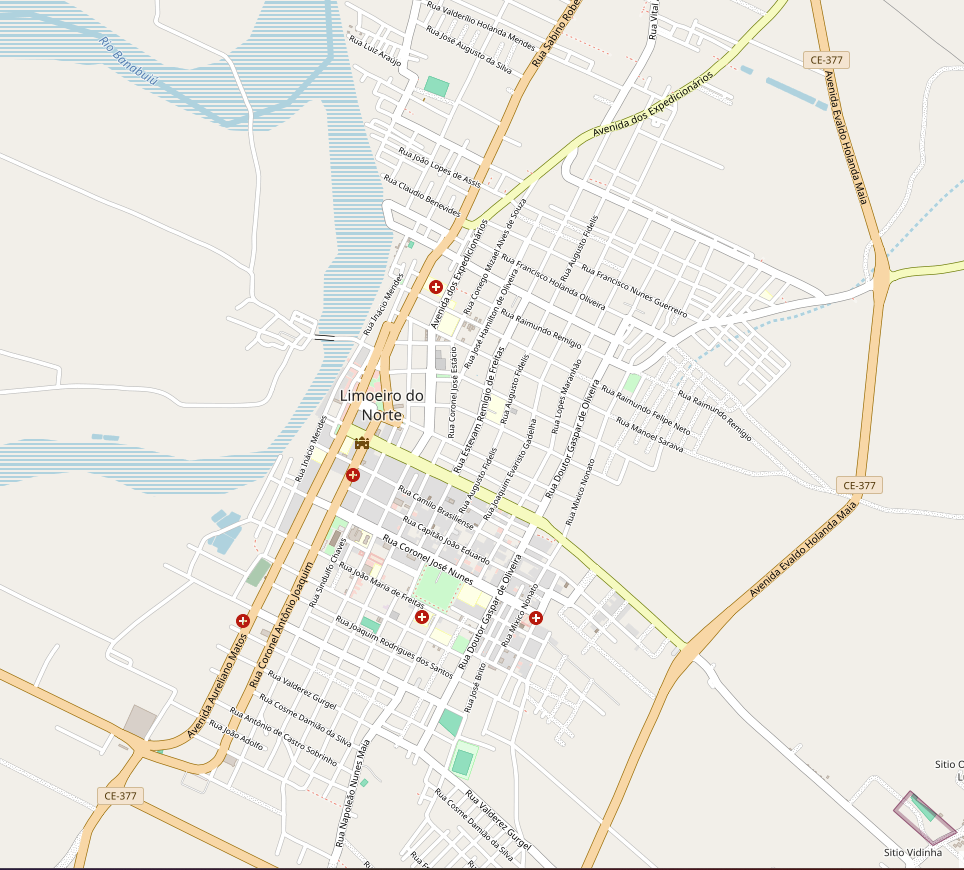
\includegraphics[width=6cm, height=5cm]{images/limoeiro-mapa.png}
    \subcaption{Map of Limoeiro downtown.}
  \end{minipage}
  \caption{\label{fig:graph-examples} Maps extracted from \gls{osm}.}
\end{figure}

Figure~\ref{fig:cases-per-status} shows the number of notifications clustered by the final classification for the entire \gls{sinan} dataset, including options such as positive for Dengue or Chikungunya, Dengue with alarm signals, severe Dengue, discarded cases and cases pending closure. According to the current health department of \textit{Alto Santo}, there was under-reporting of cases in \gls{sinan} during the initial years. This can be observed, for example, in Figure~\ref{fig:cases-per-year}, which presents the number of notifications grouped by year for each city. In \textit{Alto Santo}, in 2017, more than 200 notifications remained pending.

\begin{figure}[h!]
    \centering
    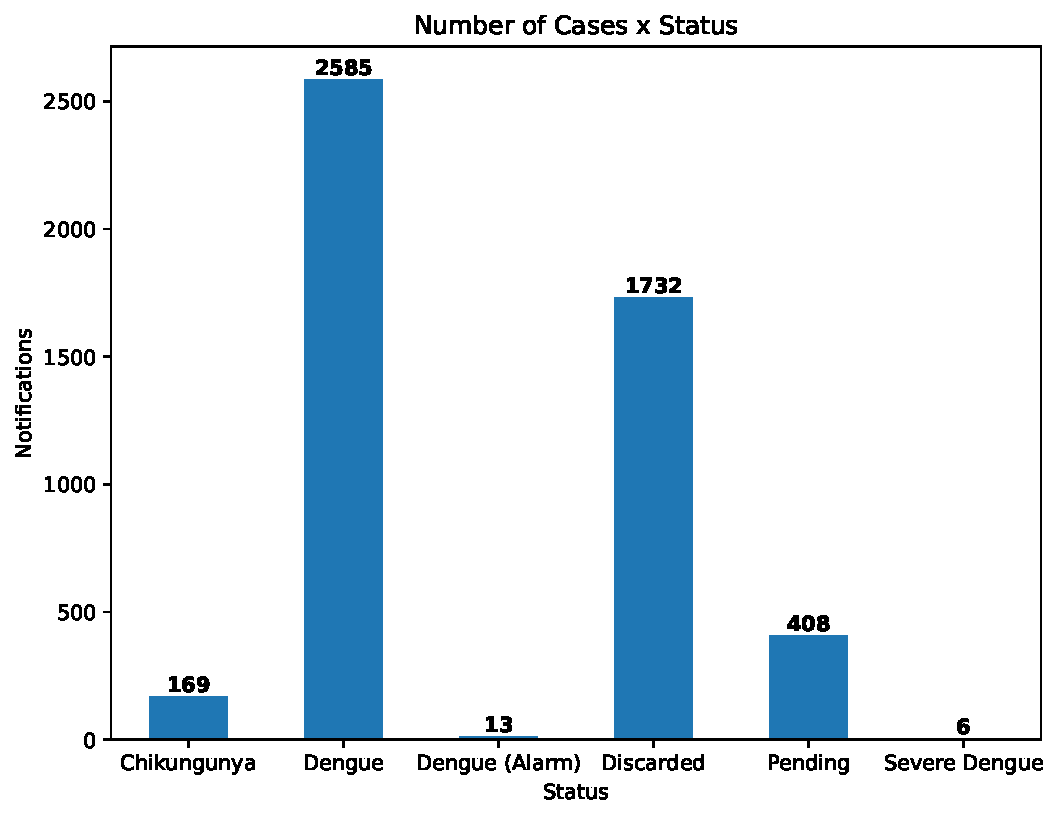
\includegraphics[width=8cm, height=7cm]{images/cases-per-status.pdf}
    \caption{Number of notifications considering both cities under study.}\label{fig:cases-per-status}
\end{figure}

Analyzing the data presented in Figure~\ref{fig:cases-per-year}, except for 2018 in \textit{Limoeiro do Norte}, there are at least 150 positive cases each year, with the highest number of cases occurring in 2019 and 2020. The year 2020 was considered an epidemic year, reporting more than 1450 positive cases. In \textit{Alto Santo}, more than half of the total notifications were reported only in 2017, with more cases pending than confirmed positive or negative. The number of positive notifications in all other years is less than 75, and almost no cases occurred in the two years after 2017. According to conversations with the \textit{Alto Santo} health department, except for 2017, none of the years was characterized as epidemic seasons. The number of cases increased only in 2021.
    
\begin{figure}[h!]
\centering
  \begin{minipage}[c]{.45\textwidth}
    \centering
    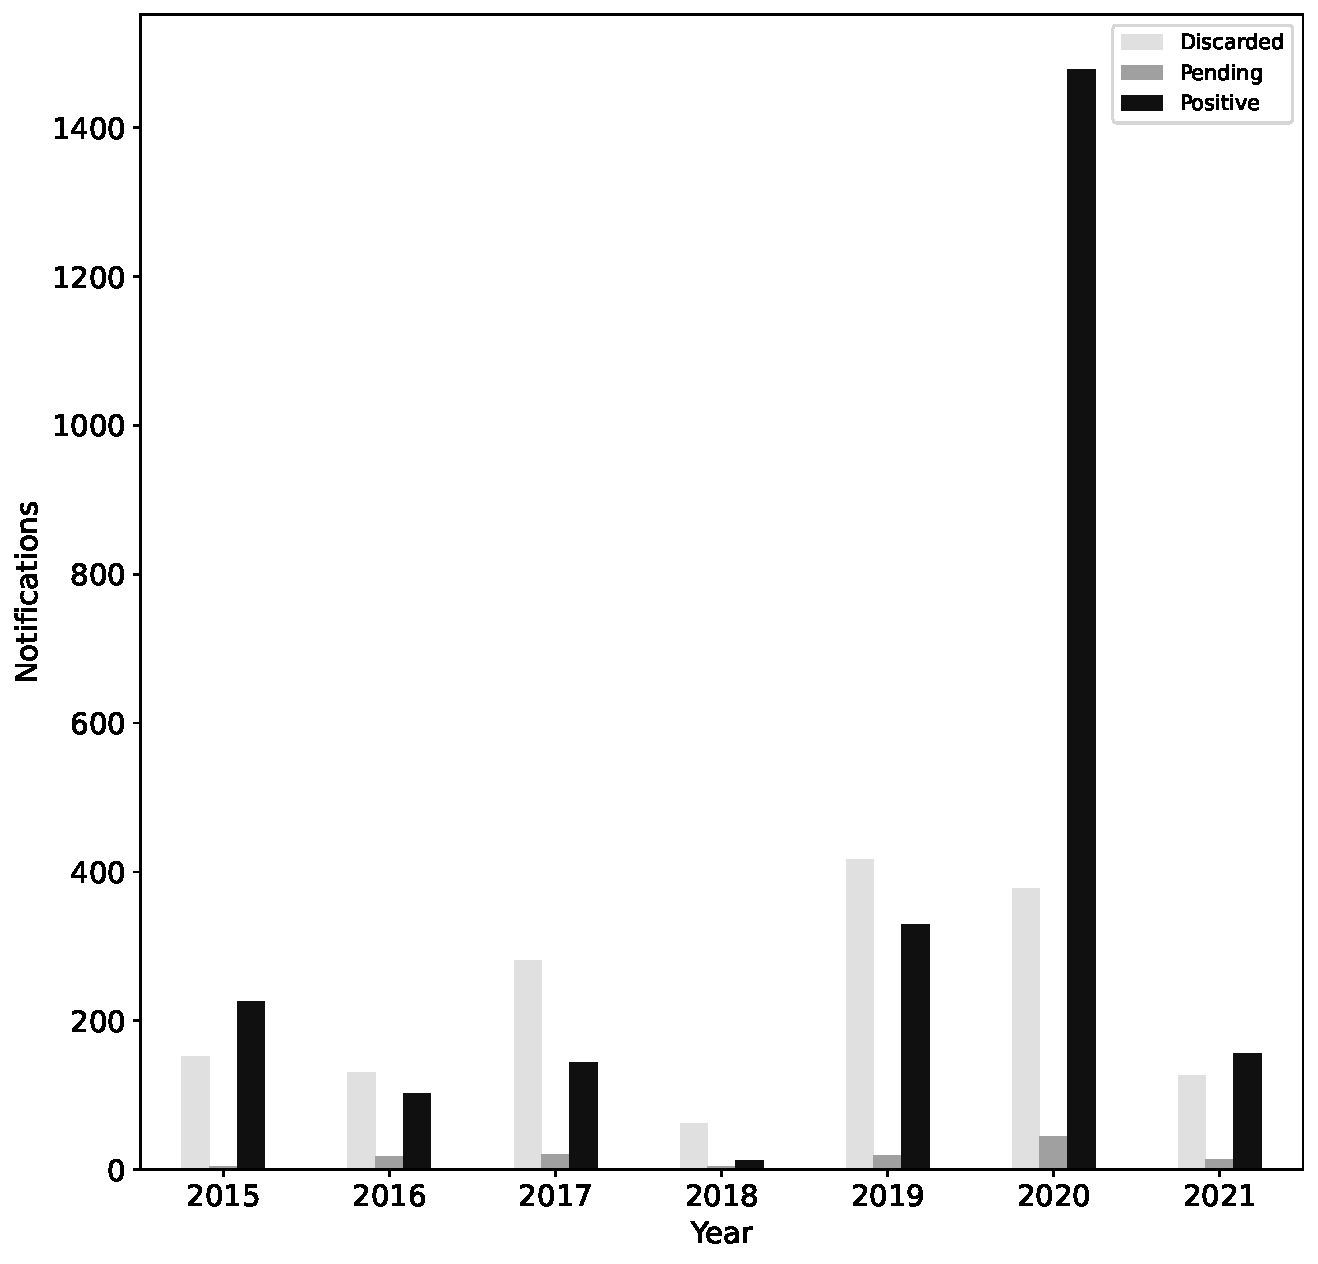
\includegraphics[width=6.5cm, height=7cm]{images/cases-per-year-Limoeiro do Norte.pdf}
    \subcaption{Notifications from Limoeiro.}
  \end{minipage}
  \hfill
  \begin{minipage}[c]{.45\textwidth}
    \centering
    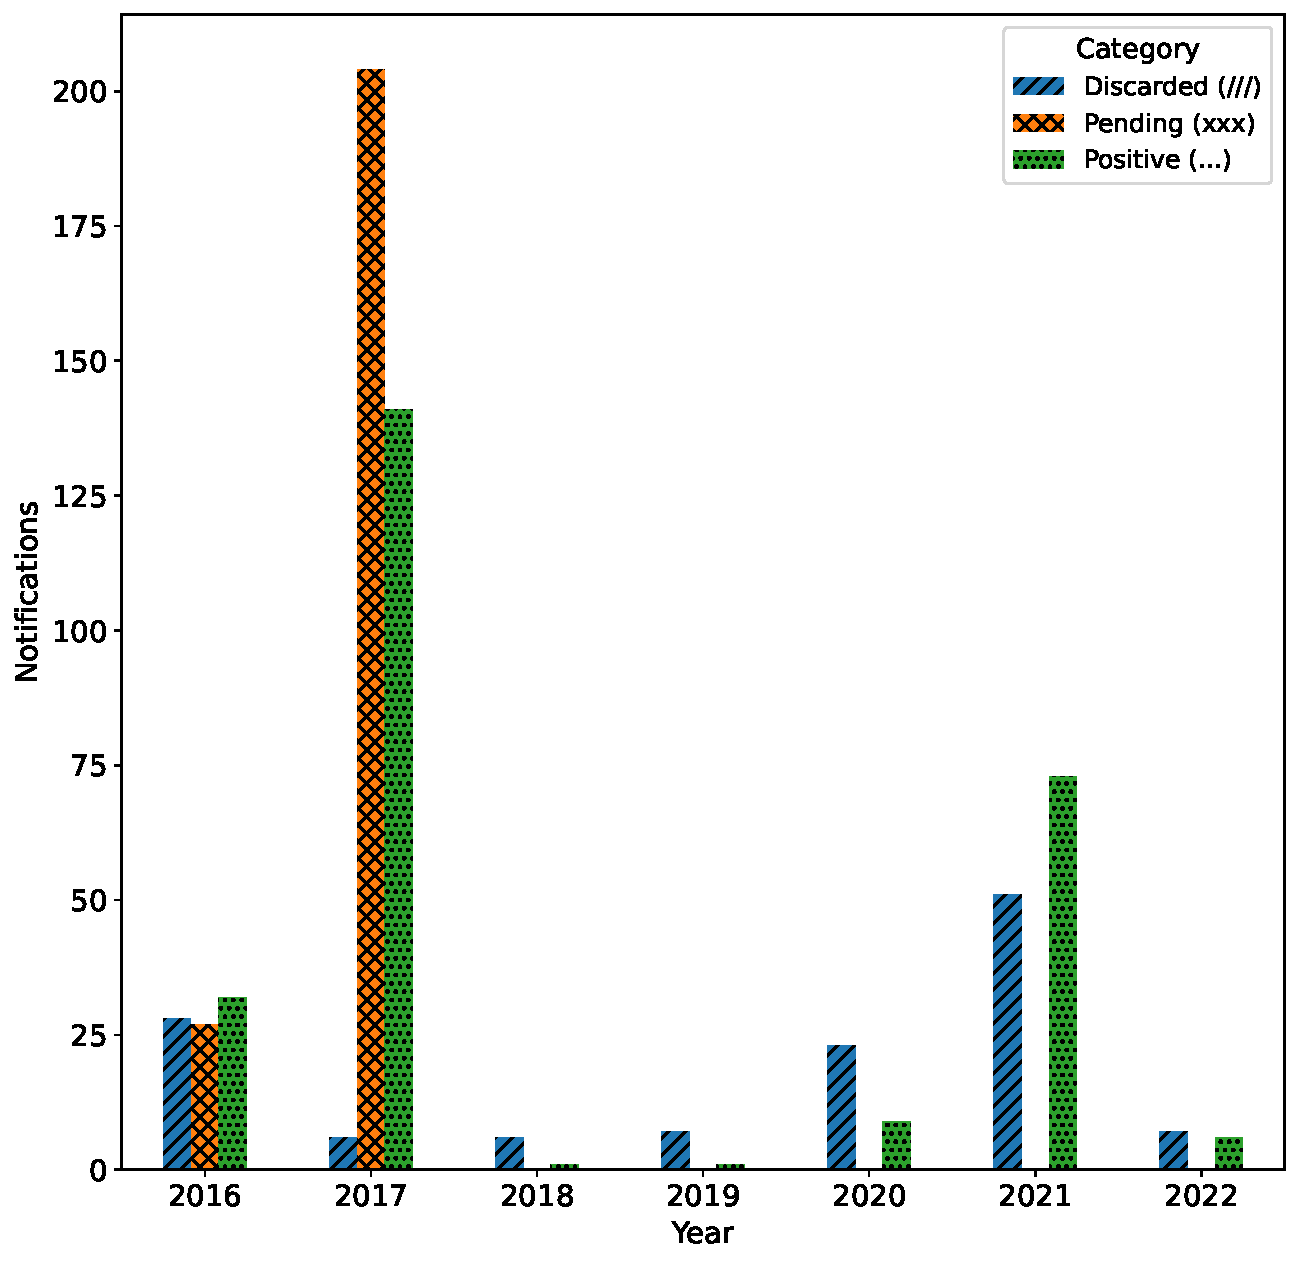
\includegraphics[width=6.5cm, height=7cm]{images/cases-per-year-Alto Santo.pdf}
    \subcaption{Notifications from Alto Santo.}
  \end{minipage}
  \caption{\label{fig:cases-per-year} Number of notifications per year.}
\end{figure}

Considering the total number of notifications and their distribution over the years, it is evident that \textit{Limoeiro do Norte}, with a larger population, also experiences a higher number of Dengue and Chikungunya cases every year. To analyze the distribution of cases in the same granularity of time used by the health departments, we selected the two years with the most notifications for each city, specifically 2019/2020 for \textit{Limoeiro} and 2017/2021 for \textit{Alto Santo} (Figures~\ref{fig:cases-per-week-limoeiro} and~\ref{fig:cases-per-week-as}, respectively). These figures depict the distribution of notifications for each \gls{ew} with at least one notification.
  
\begin{figure}[h!]
  \begin{minipage}[c]{.9\textwidth}
    \centering
    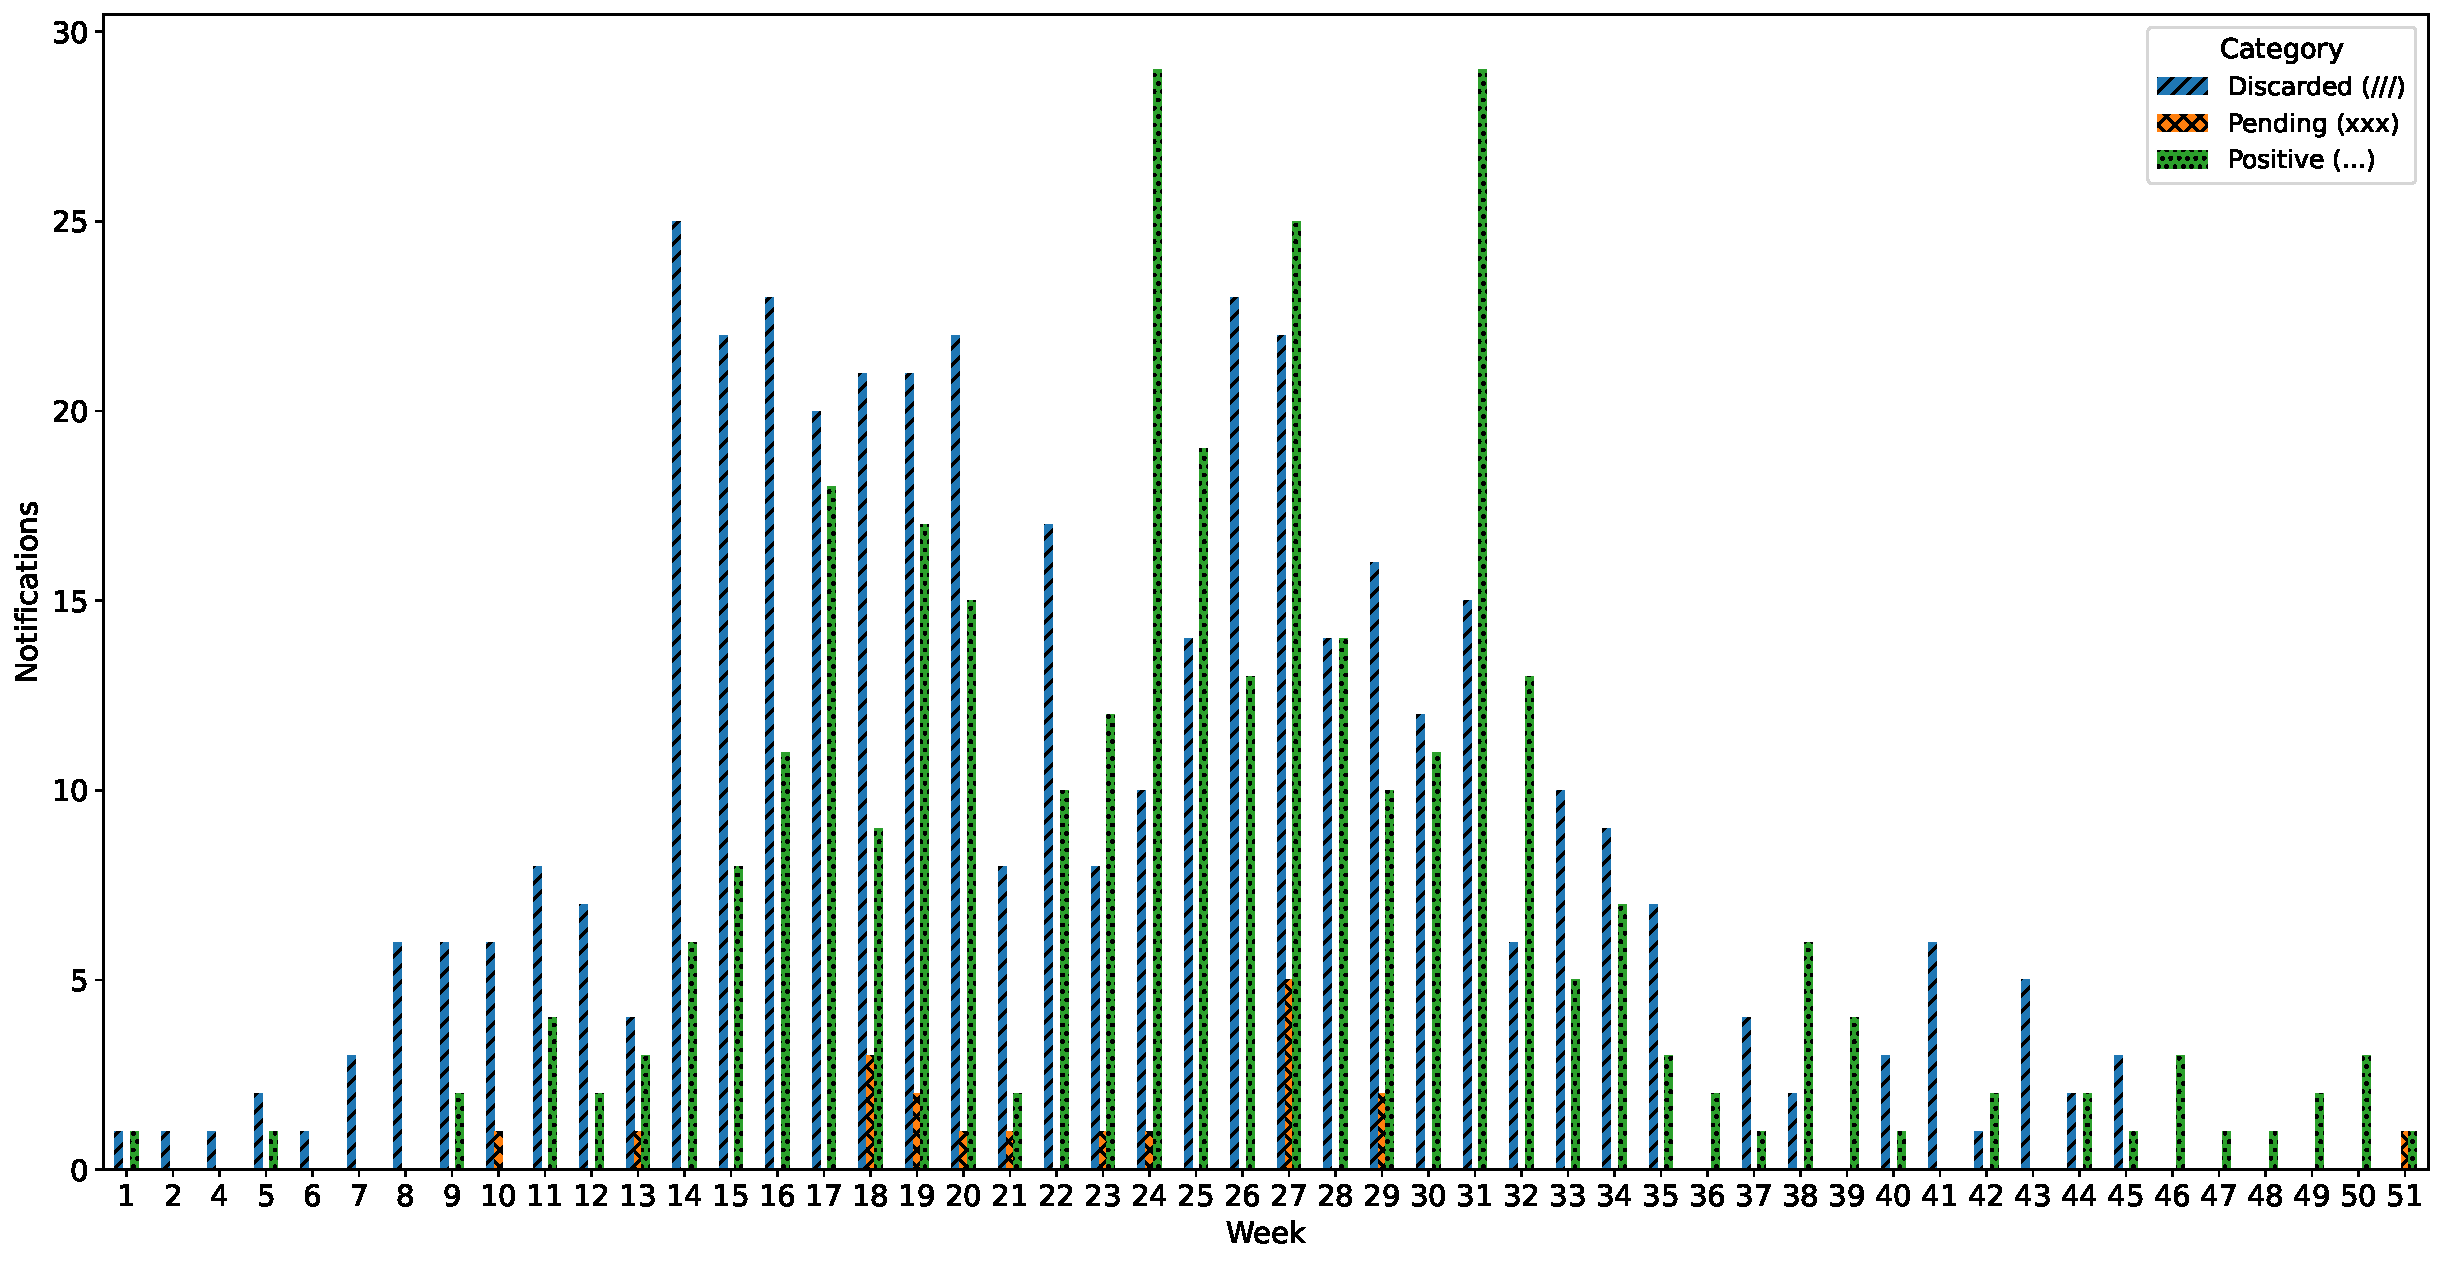
\includegraphics[scale=0.32]{images/cases-per-week--2019-Limoeiro do Norte.pdf}
    \subcaption{Notifications from Limoeiro - 2019.}
  \end{minipage}
  \\
  \begin{minipage}[c]{.9\textwidth}
    \centering
    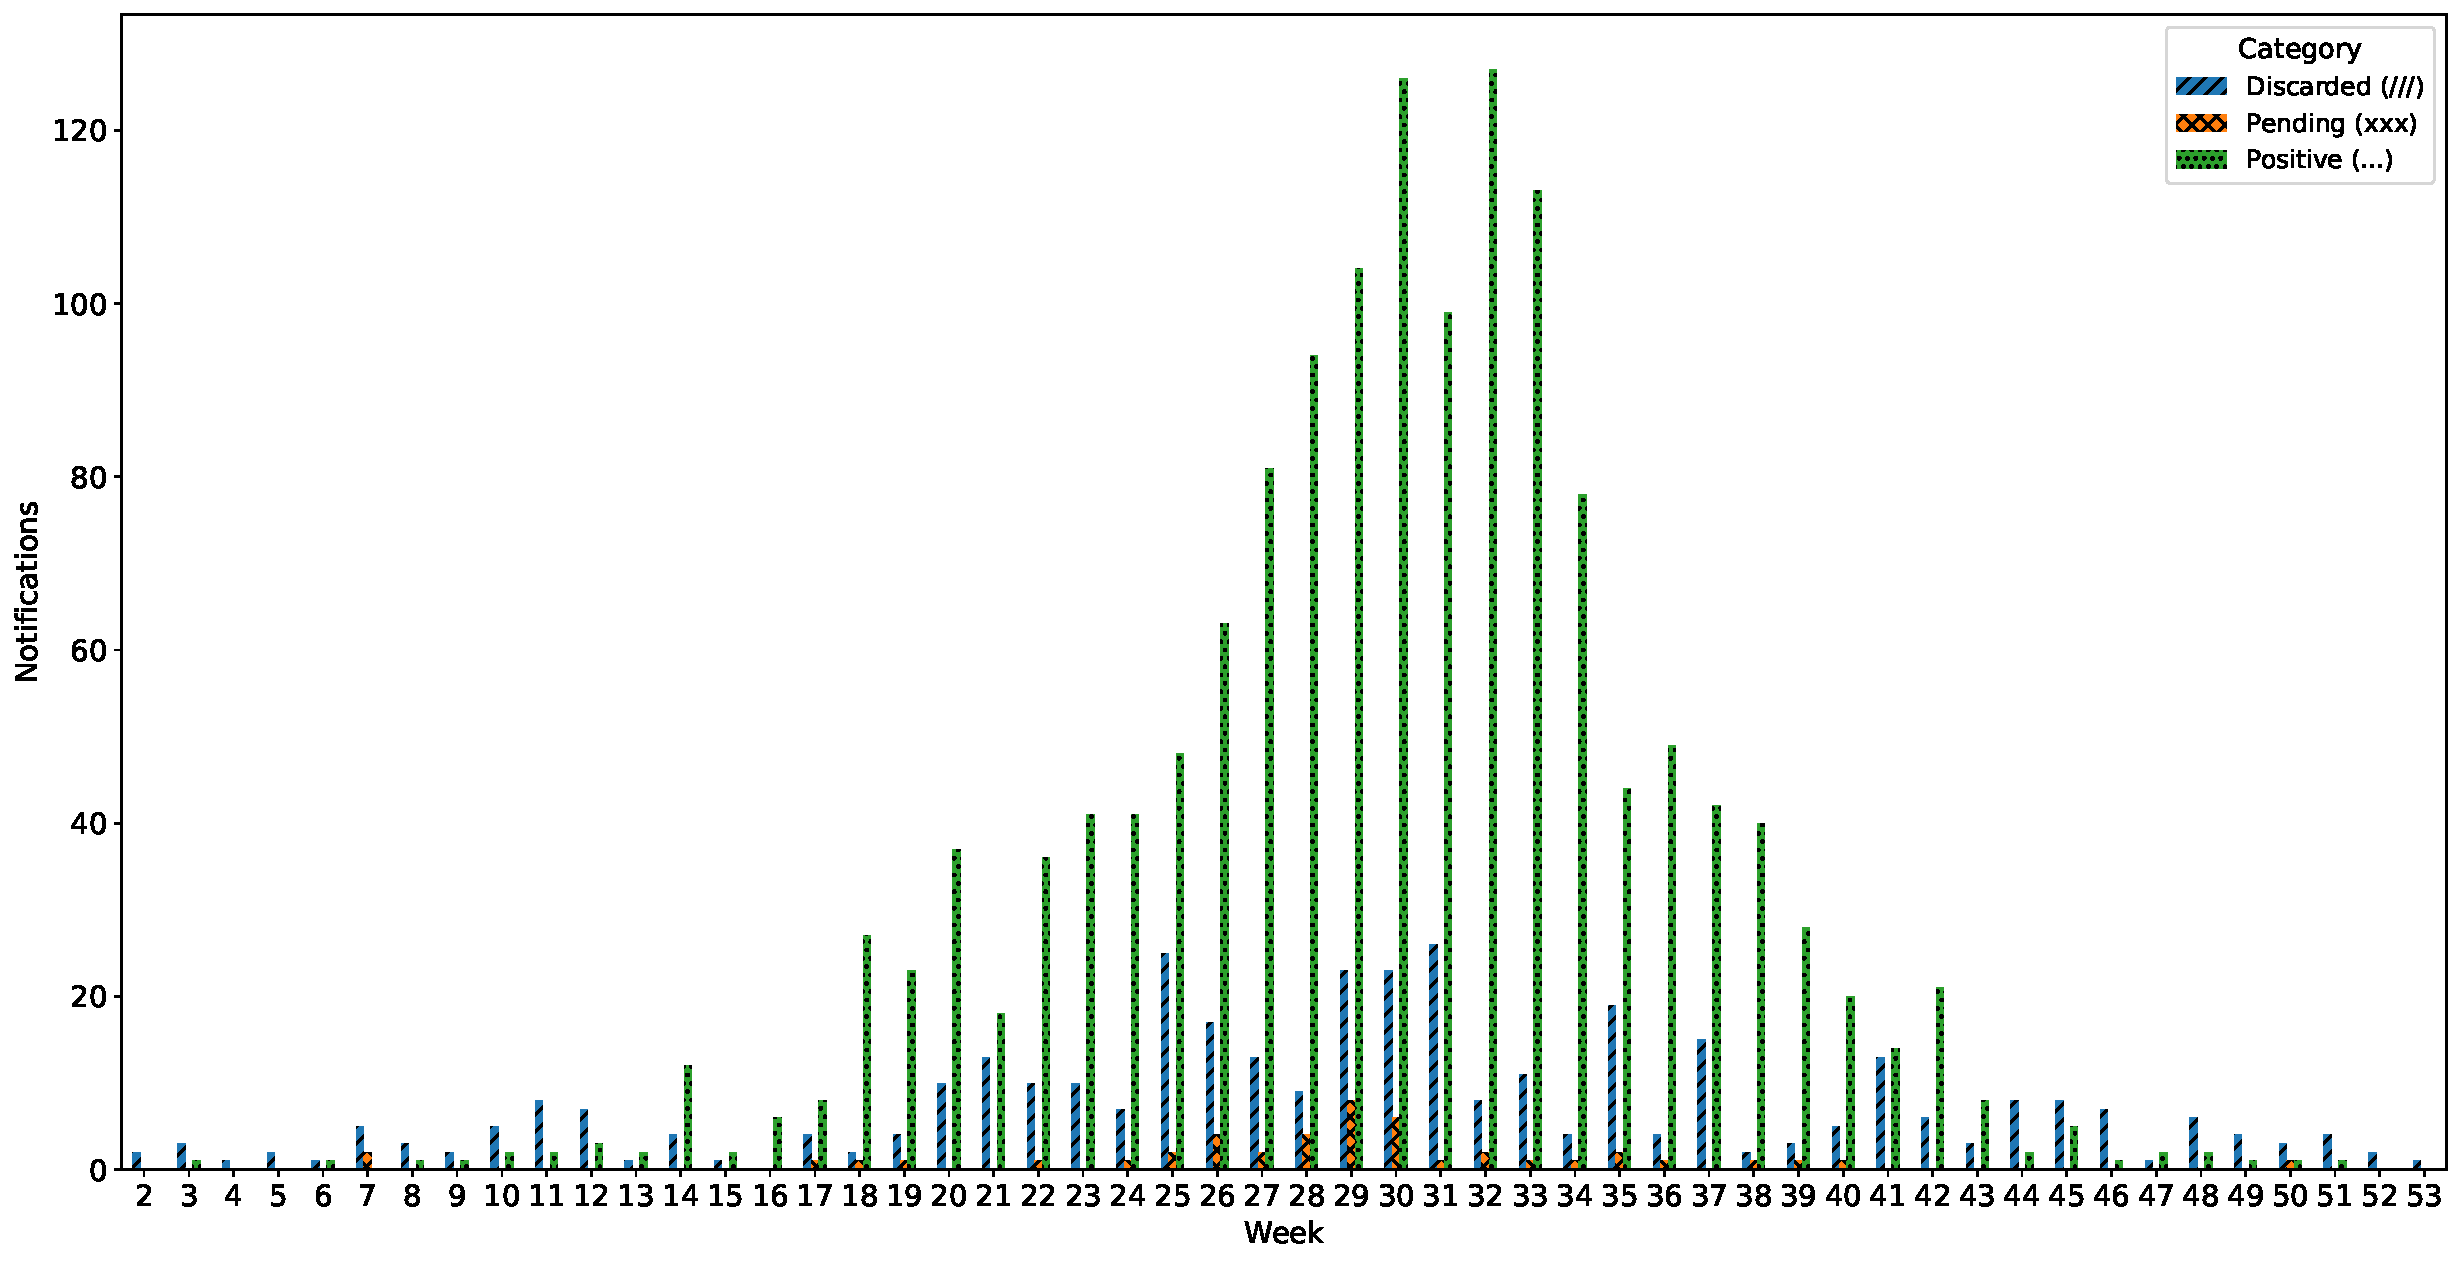
\includegraphics[scale=0.32]{images/cases-per-week--2020-Limoeiro do Norte.pdf}
    \subcaption{Notifications from Limoeiro - 2020.}
  \end{minipage}
  \caption{\label{fig:cases-per-week-limoeiro} Number of notifications per week - Limoeiro do Norte.}
\end{figure}

\begin{figure}[h!]
  \begin{minipage}[c]{.9\textwidth}
    \centering
    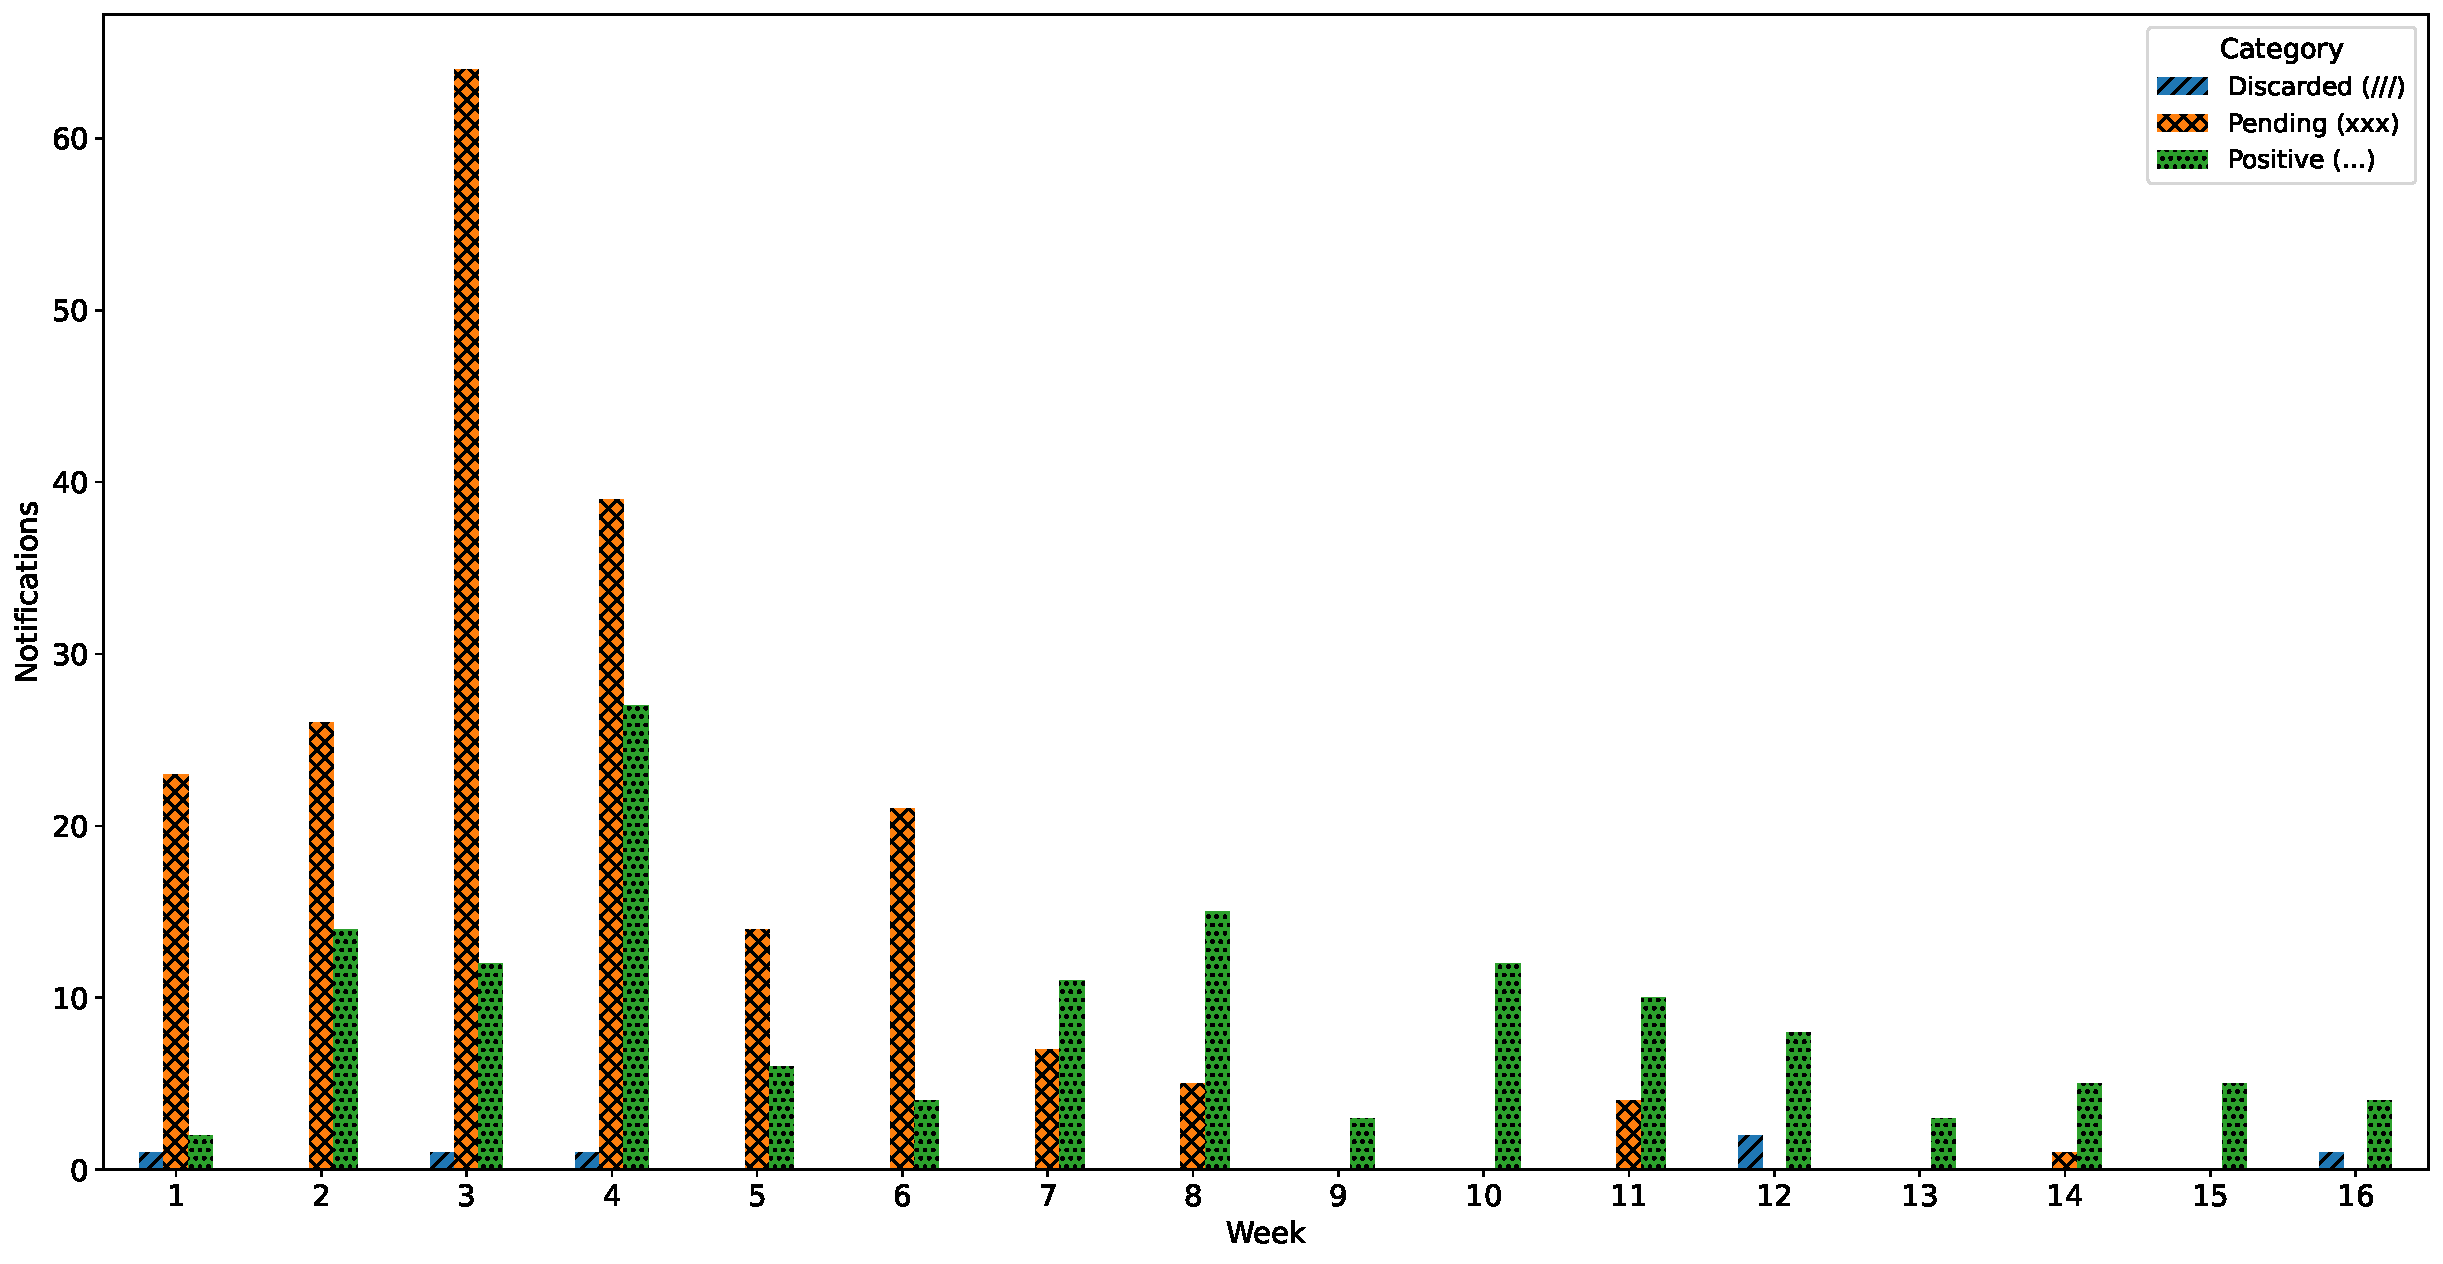
\includegraphics[scale=0.32]{images/cases-per-week--2017-Alto Santo.pdf}
    \subcaption{Notifications from Alto Santo - 2017.}
  \end{minipage}
  \\
  \begin{minipage}[c]{.9\textwidth}
    \centering
    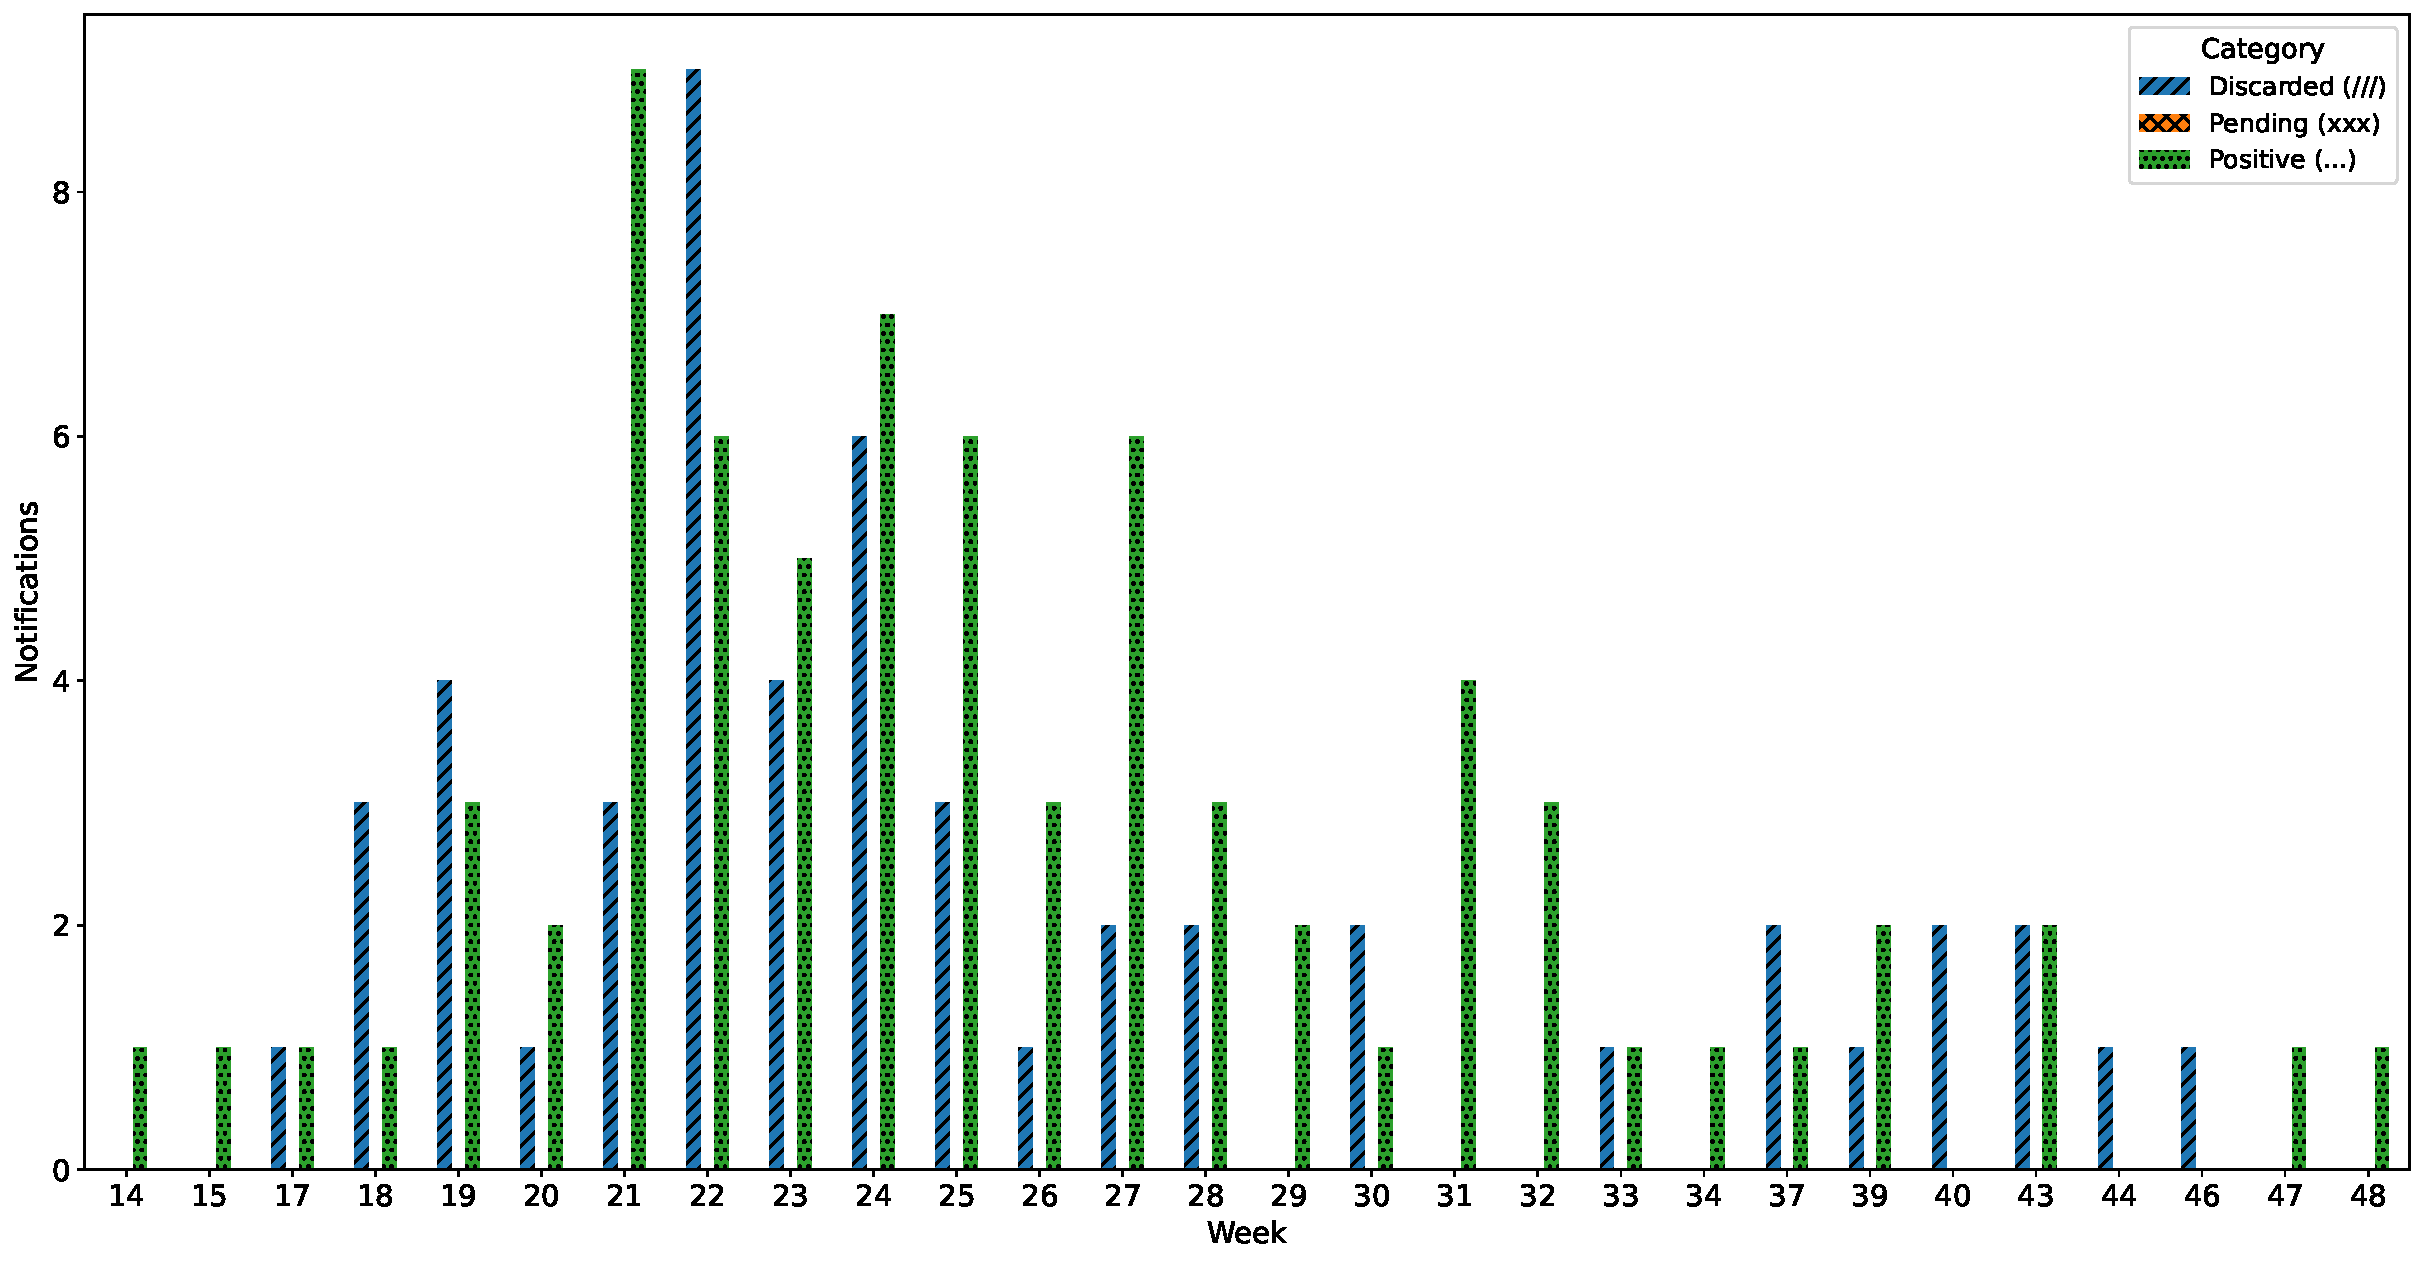
\includegraphics[scale=0.32]{images/cases-per-week--2021-Alto Santo.pdf}
    \subcaption{Notifications from Alto Santo - 2021.}
  \end{minipage}
  \caption{\label{fig:cases-per-week-as} Number of notifications per week - Alto Santo.}
\end{figure}

In \textit{Alto Santo}, during 2017, dengue cases were reported within the first 16 epidemiological weeks (\gls{ews}), peaking at 25 cases in week 4. Based on the application, we can classify these notifications as either positive or negative, given the high number of confirmed dengue cases during the same period. In 2021, cases were recorded between \gls{ew} 14 and 48, with a lower weekly incidence, reaching a peak of 9 confirmed cases in week 21.

From \textit{Limoeiro}, in 2019, cases are present in almost all weeks with peaks of positive cases occurring between weeks 24 and 32, ranging from 10 to 29 cases. There is an epidemic season from weeks 20 to 38 of 2020, where the number of cases is at least 40, and for 8 consecutive weeks after the 27 \gls{ew}, the number of cases ranges from 80 to 123.

Two points need to be highlighted to understand this dataset. 
First, underreporting likely occurred as infected individuals may not have pursued hospital care due to: \textit{(1)} Knowing Dengue is seasonal, individuals often self-diagnose when experiencing common disease symptoms, \textit{(2)} adherence to clinically recommended protocols without formal testing, or \textit{(3)} mild symptoms that did not disrupt daily activities. Second, the absence of spatiotemporal records on vector-control interventions (e.g., insecticide campaigns and larval habitat removal) obscures their impact on mosquito populations and localized transmission dynamics. These limitations collectively contribute to the observed fluctuations in notifications.

In both cities, public health strategies lack integration with digital surveillance tools or predictive systems. Unfortunately, they rely on reactive containment measures initiated only after spikes in confirmed dengue cases. This firefighting approach, common in resource-constrained municipalities in Brazil, fails to optimize prevention due to three key gaps: \textit{(i)} delayed detection of epidemiological trends, \textit{(ii)} absence of data-driven risk mapping to prioritize high-risk zones, and \textit{(iii)} ad hoc resource allocation that overlooks transmission dynamics. Consequently, interventions often occur too late to effectively curb outbreaks, perpetuating cycles of suboptimal public health outcomes.

\section{Instance Generation}\label{sec:instance-generation}

To identify (label) each city block, we employ a graph-theoretical procedure
that corresponds to finding the faces of a planar
embedding~\citep{diestel2024graph}. A planar embedding, also called a rotation
system, is defined for a planar graph by assigning, for each vertex $( i \in V
	)$, a cyclic ordering $C(i)$ of its neighbors (typically in clockwise order).
Intuitively, this defines the clockwise order of streets around each
intersection. This rotation system can be computed using the geometric slope of
each incident arc~\citep{PhilipKleinShayMozes}. As an illustrative example,
consider the graph in \ref{fig:non_isolated_nodes}. Its planar embedding can be
described by the function $C$ as shown in Table~\ref{tabnew}.

\begin{figure}[ht!]
	\centering
	\begin{tikzpicture}[>=latex]
		% nodes
		% block A
		\coordinate (A1) at (0.1, 2.9);
		\coordinate (A2) at (1.9, 2.9);
		\coordinate (A3) at (1.9, 2);
		\coordinate (A4) at (1.9, 1.1);
		\coordinate (A5) at (0.1, 1.1);
		\coordinate (BorderA1) at (0, 3);
		\coordinate (BorderA2) at (2, 3);
		\coordinate (BorderA3) at (2, 2);
		\coordinate (BorderA4) at (2, 1);
		\coordinate (BorderA5) at (0, 1);
		% block B
		\coordinate (B1) at (2.1, 2.9);
		\coordinate (B2) at (3.9, 2.9);
		\coordinate (B3) at (3.9, 1.1);
		\coordinate (B4) at (2.1, 1.1);
		\coordinate (B5) at (2.1, 2);
		\coordinate (BorderB1) at (2, 3);
		\coordinate (BorderB2) at (4, 3);
		\coordinate (BorderB3) at (4, 1);
		\coordinate (BorderB4) at (2, 1);
		\coordinate (BorderB5) at (2, 2);
		% block C
		\coordinate (C1) at (2, 0.9);
		\coordinate (C2) at (2.9, 0.1);
		\coordinate (C3) at (1.1, 0.1);
		\coordinate (BorderC1) at (2, 1);
		\coordinate (BorderC2) at (3.1, 0);
		\coordinate (BorderC3) at (0.9, 0);
		% block B
		\coordinate (D1) at (2, 3.1);
		\coordinate (D2) at (1.1, 3.9);
		\coordinate (D3) at (2.9, 3.9);
		\coordinate (BorderD1) at (2, 3);
		\coordinate (BorderD2) at (0.9, 4);
		\coordinate (BorderD3) at (3.1, 4);
		% blocks
		\def\blockA{A1, A2, A3, A4, A5}
		\def\blockB{B1, B2, B3, B4, B5}
		\def\blockC{C1, C2, C3}
		\def\blockD{D1, D2, D3}
		% arcs
		\def\arcs{%
			% block A
			BorderA1 BorderA2
			BorderA2 BorderA3
			BorderA3 BorderA4
			BorderA4 BorderA5
			BorderA5 BorderA1
			% block B
			BorderB1 BorderB2
			BorderB2 BorderB3
			BorderB3 BorderB4
			BorderB4 BorderB5
			BorderB5 BorderB1
			% block C
			BorderC1 BorderC2
			BorderC2 BorderC3
			BorderC3 BorderC1
			% block D
			BorderD1 BorderD2
			BorderD2 BorderD3
			BorderD3 BorderD1
		}
		\readarray\arcs\Arcs[16,2]
		% print arcs
		\drawArcs{\Arcs}{\ArcsROWS}{->, gray!20, to path={-| (\tikztotarget)}}
		%block A
		\drawBlock{A1}{\blockA}{red!50};
		%block B
		\drawBlock{B1}{\blockB}{black!50};
		%block C
		\drawBlock{C1}{\blockC}{yellow!50};
		%block D
		\drawBlock{D1}{\blockD}{blue!50};
		% dot
		\filldraw[black] (BorderD1) circle (1pt);
		% blocks labels
		% A
		\node[xshift=2mm, yshift=-1.5mm] at (0.8, 2.2) {$b_1$};
		\node[xshift=2mm, yshift=-1.5mm] at (A1) {\tiny$b_1^1$};
		\node[xshift=-2mm, yshift=-1.5mm] at (A2) {\tiny$b_1^2$};
		\node[xshift=-2mm, yshift=1.5mm] at (A3) {\tiny$b_1^3$};
		\node[xshift=-2mm, yshift=1.5mm] at (A4) {\tiny$b_1^4$};
		\node[xshift=2mm, yshift=1.5mm] at (A5) {\tiny$b_1^5$};
		% B
		\node[xshift=2mm, yshift=-1.5mm] at (2.8, 2.2) {$b_2$};
		\node[xshift=2mm, yshift=-1.5mm] at (B1) {\tiny$b_2^1$};
		\node[xshift=-2mm, yshift=-1.5mm] at (B2) {\tiny$b_2^2$};
		\node[xshift=-2mm, yshift=1.5mm] at (B3) {\tiny$b_2^3$};
		\node[xshift=2mm, yshift=1.5mm] at (B4) {\tiny$b_2^4$};
		\node[xshift=2mm, yshift=1.5mm] at (B5) {\tiny$b_2^5$};
		% C
		\node[xshift=2mm, yshift=-1.5mm] at (1.8, 0.5) {$b_3$};
		\node[yshift=-1.5mm] at (C1) {\tiny$b_3^1$};
		\node[xshift=-4mm, yshift=1.5mm] at (C2) {\tiny$b_3^2$};
		\node[xshift=4mm, yshift=1.5mm] at (C3) {\tiny$b_3^3$};
		% B
		\node[xshift=2mm, yshift=-1.5mm] at (1.8, 3.85) {$b_4$};
		\node[yshift=2.5mm] at (D1) {\tiny$b_4^1$};
		\node[xshift=4.5mm, yshift=-1.5mm] at (D2) {\tiny$b_4^2$};
		\node[xshift=-4.5mm, yshift=-1.5mm] at (D3) {\tiny$b_4^3$};
	\end{tikzpicture}
	\caption{Example of non-isolated street-blocks.}
	\label{fig:non_isolated_nodes}
\end{figure}

\begin{table}[h!]
	\centering
	\caption{Connections for each city block}\label{tabnew}
	\begin{tabular}{cl}
		\hline
		\textbf{City Block} & \textbf{Connections}                      \\ \hline
		\( C(b^1_1) \)      & \( (b^5_1, b^2_1) \)                      \\
		\( C(b^2_1) \)      & \( (b^3_1, b^1_1, b^2_4, b^3_4, b^2_2) \) \\
		\( C(b^3_1) \)      & \( (b^4_1, b^1_2) \)                      \\
		\( C(b^4_1) \)      & \( (b^3_3, b^5_1, b^5_2, b^3_2, b^2_3) \) \\
		\( C(b^5_1) \)      & \( (b^1_1, b^4_1) \)                      \\
		\( C(b^2_2) \)      & \( (b^1_2, b^3_2) \)                      \\
		\( C(b^3_2) \)      & \( (b^4_2, b^2_2) \)                      \\
		\( C(b^2_3) \)      & \( (b^3_3, b^1_3) \)                      \\
		\( C(b^3_3) \)      & \( (b^1_3, b^2_3) \)                      \\
		\( C(b^2_4) \)      & \( (b^3_4, b^1_4) \)                      \\
		\( C(b^3_4) \)      & \( (b^1_4, b^2_4) \)                      \\ \hline
	\end{tabular}
\end{table}

With combinatorial embedding \( C \) and arc set \( A \), we identify all bounded and unbounded faces of the planar graph using a traversal procedure formalized in Algorithm~\ref{alg:find_faces}. Each face corresponds to a cyclic sequence of arcs that form the boundary of a region enclosed by streets (i.e., a city block). The algorithm iteratively traverses unused arcs in the graph by following the clockwise ordering defined by \( C \), marking each arc as visited once it has been assigned to a face. Each traversal terminates upon returning to the starting arc, thus completing a cycle (face). This procedure ensures that every face is uniquely defined by a sequence of arcs traversed in the clockwise direction relative to the embedding. We note that every planar embedding has one unbounded `outer' face encircling the whole graph. This outer face does not correspond to any physical city block, so we exclude it from the set of labeled blocks.

\begin{algorithm}[h!]
\caption{Face-finding Algorithm for Planar Embedding}\label{alg:find_faces}
\KwIn{Planar graph $D = (V, A)$, combinatorial embedding $C$}
\KwOut{Set of directed cycles $\mathcal{F}$ representing faces}
\BlankLine

$\mathcal{F} \gets \emptyset$\;
Mark all arcs in $A$ as unvisited\;

\ForEach{unvisited arc $a = (u, v) \in A$}{
    $a_0 \gets a$\;
    Mark $a$ as visited\;
    $f \gets \emptyset$\;

    \Repeat{$a = a_0$}{
        Append $a$ to $f$\;
        $w \gets$ next vertex after $u$ in $C(v)$ (clockwise successor of $u$)\;
        $a \gets (v, w)$\;
        Mark $a$ as visited\;
        $u \gets v$, $v \gets w$\;
    }

    $\mathcal{F} \gets \mathcal{F} \cup \{f\}$\;
}

\Return $\mathcal{F}$\;
\end{algorithm}

\subsection{Real-case Instances}\label{subsec:real_instances}

The municipal health departments of Alto Santo and Limoeiro do Norte, located in the state of Ceará, Brazil, provided real-world dengue notification data from 2015 to 2021. The data were extracted from the \gls{sinan}~\cite{laguardia:2004}. During this period, Alto Santo reported 582 cases (2016-2021), and Limoeiro do Norte reported 4,243 cases (2015-2021), totaling 4,825 confirmed dengue cases between the two cities. The addresses of reported cases were geolocated using the OSMnx library~\cite{boeing:2017}, which provided latitude and longitude coordinates. Each case was mapped to its corresponding city block, allowing us to integrate the case data with the street network. Figure~\ref{fig:graph-examples} illustrates both the geographic maps and the corresponding graph models of Alto Santo and Limoeiro do Norte, as derived from \gls{osm}. 

\begin{figure}[h!]
	\begin{minipage}[c]{.49\textwidth}
		\centering
		\subfloat[Map of Alto Santo from OSM.]{\label{fig:altosanto}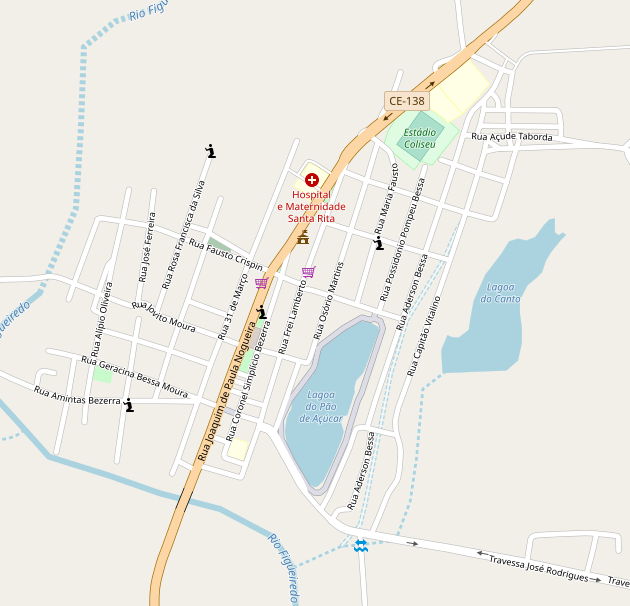
\includegraphics[width=7cm, height=6cm]{images/alto-santo-osm.png}}
	\end{minipage}%
	\begin{minipage}[c]{.49\textwidth}
		\centering
		\subfloat[Map of Limoeiro do Norte from OSM.]{\label{fig:limoeiro}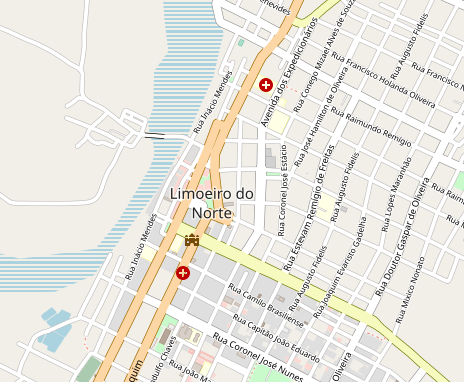
\includegraphics[width=7cm, height=6cm]{images/limoeiro-osm.png}}
	\end{minipage}\\[2mm]
	\begin{minipage}[c]{.49\textwidth}
		\centering
		\subfloat[Graph of Alto Santo.]{\label{fig:Galtosanto}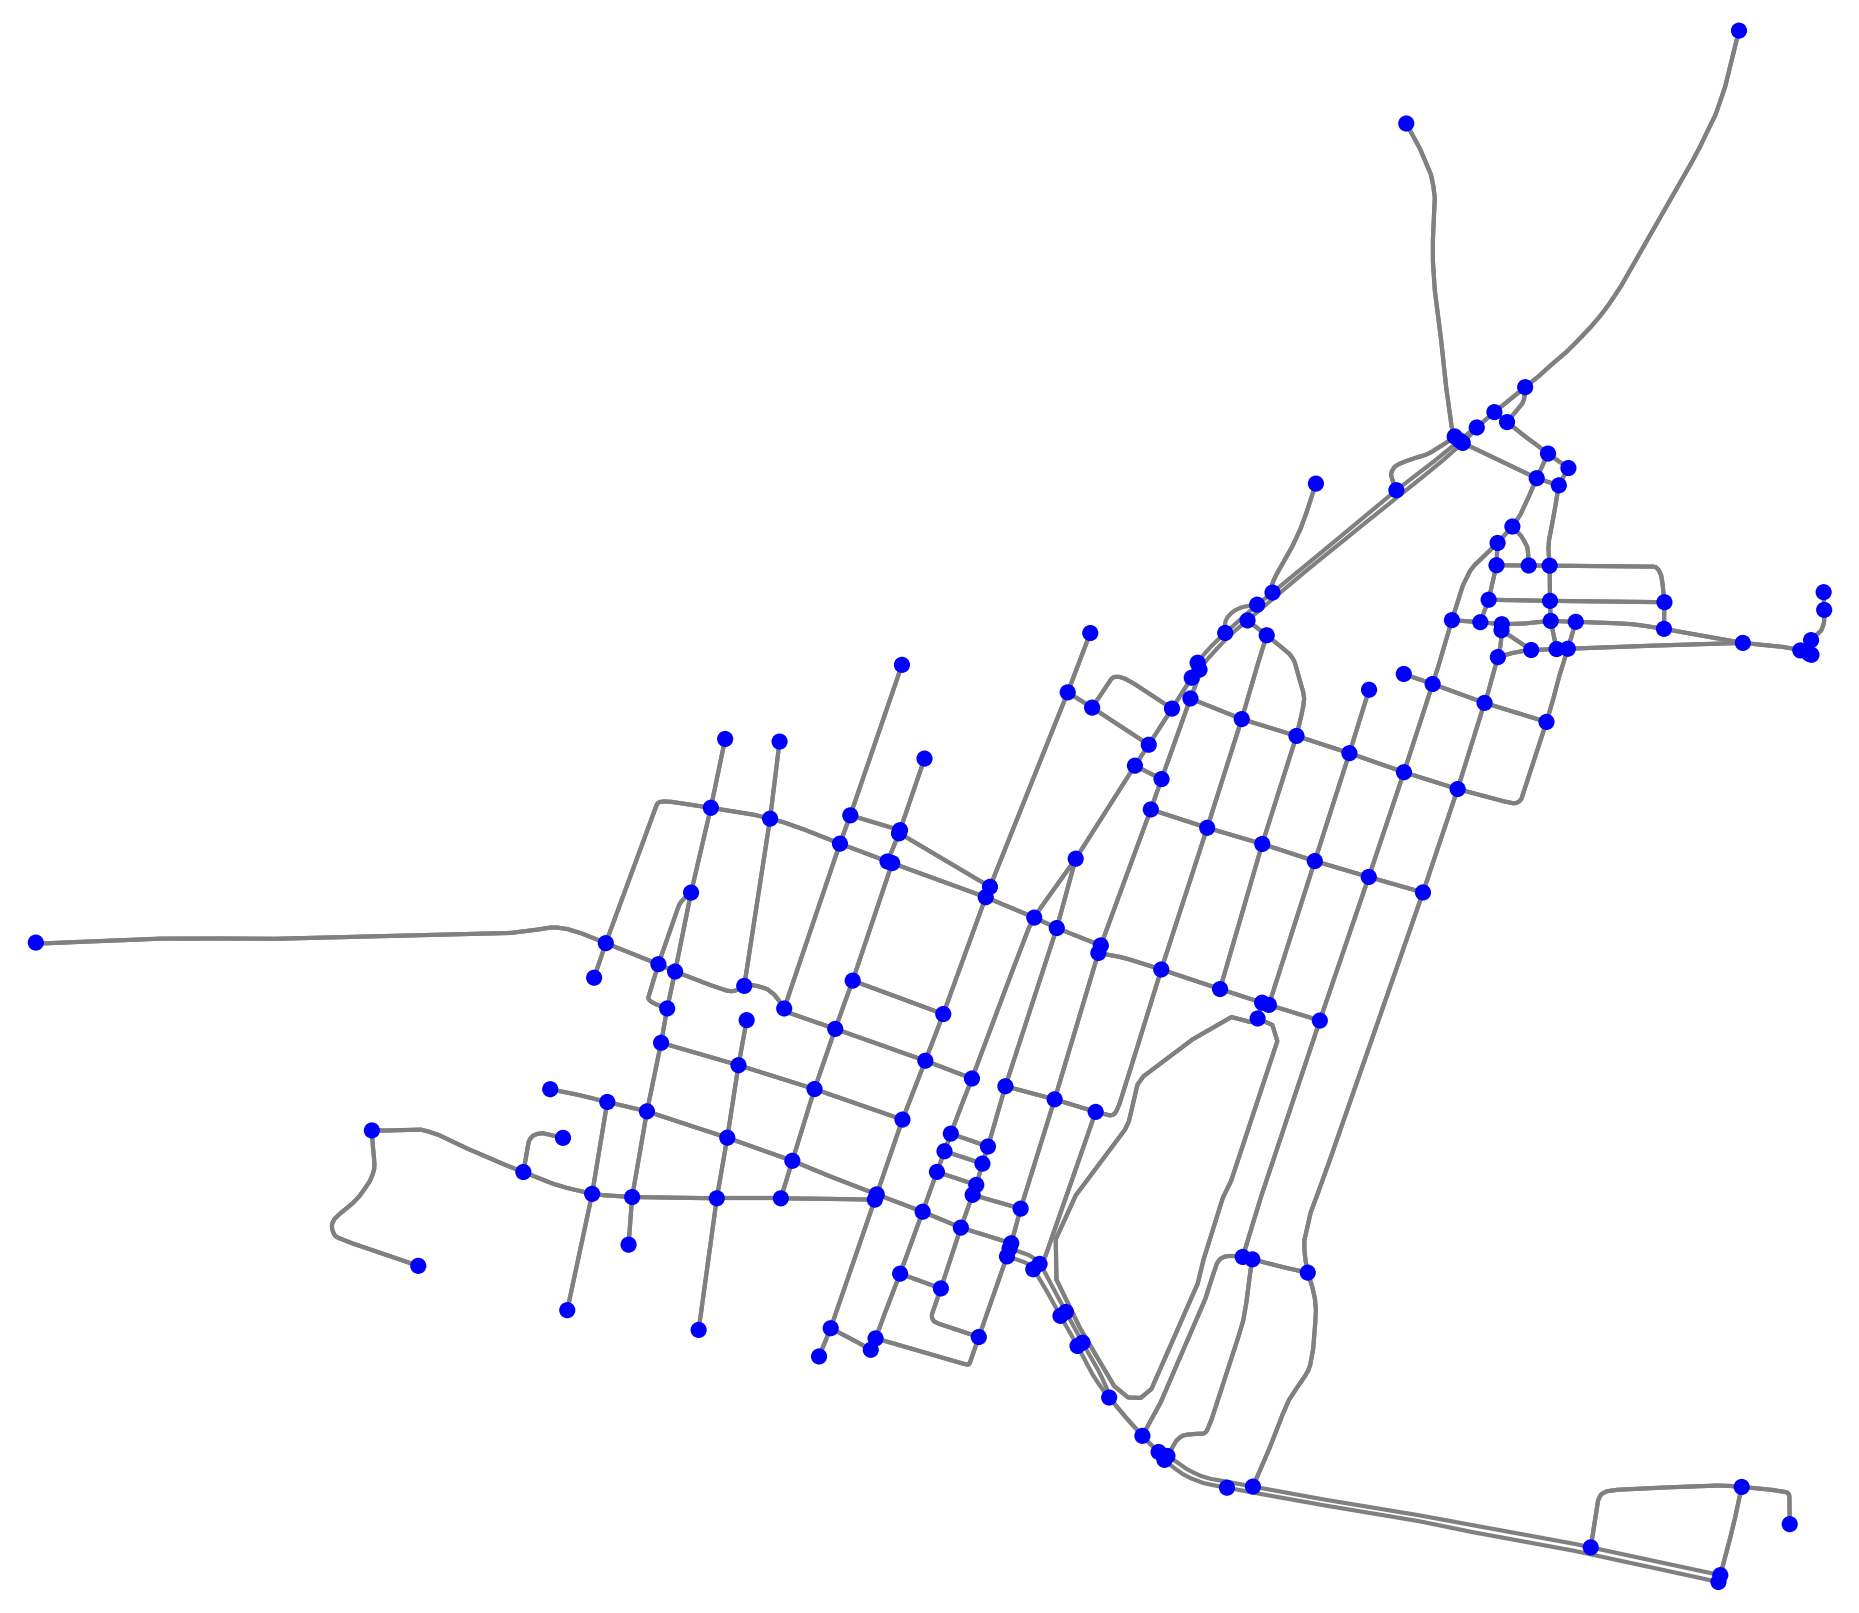
\includegraphics[width=7cm, height=6cm]{images/graph-alto-santo.png}}
	\end{minipage}%
	\begin{minipage}[c]{.49\textwidth}
		\centering
		\subfloat[Graph of Limoeiro do Norte.]{\label{fig:Glimoeiro}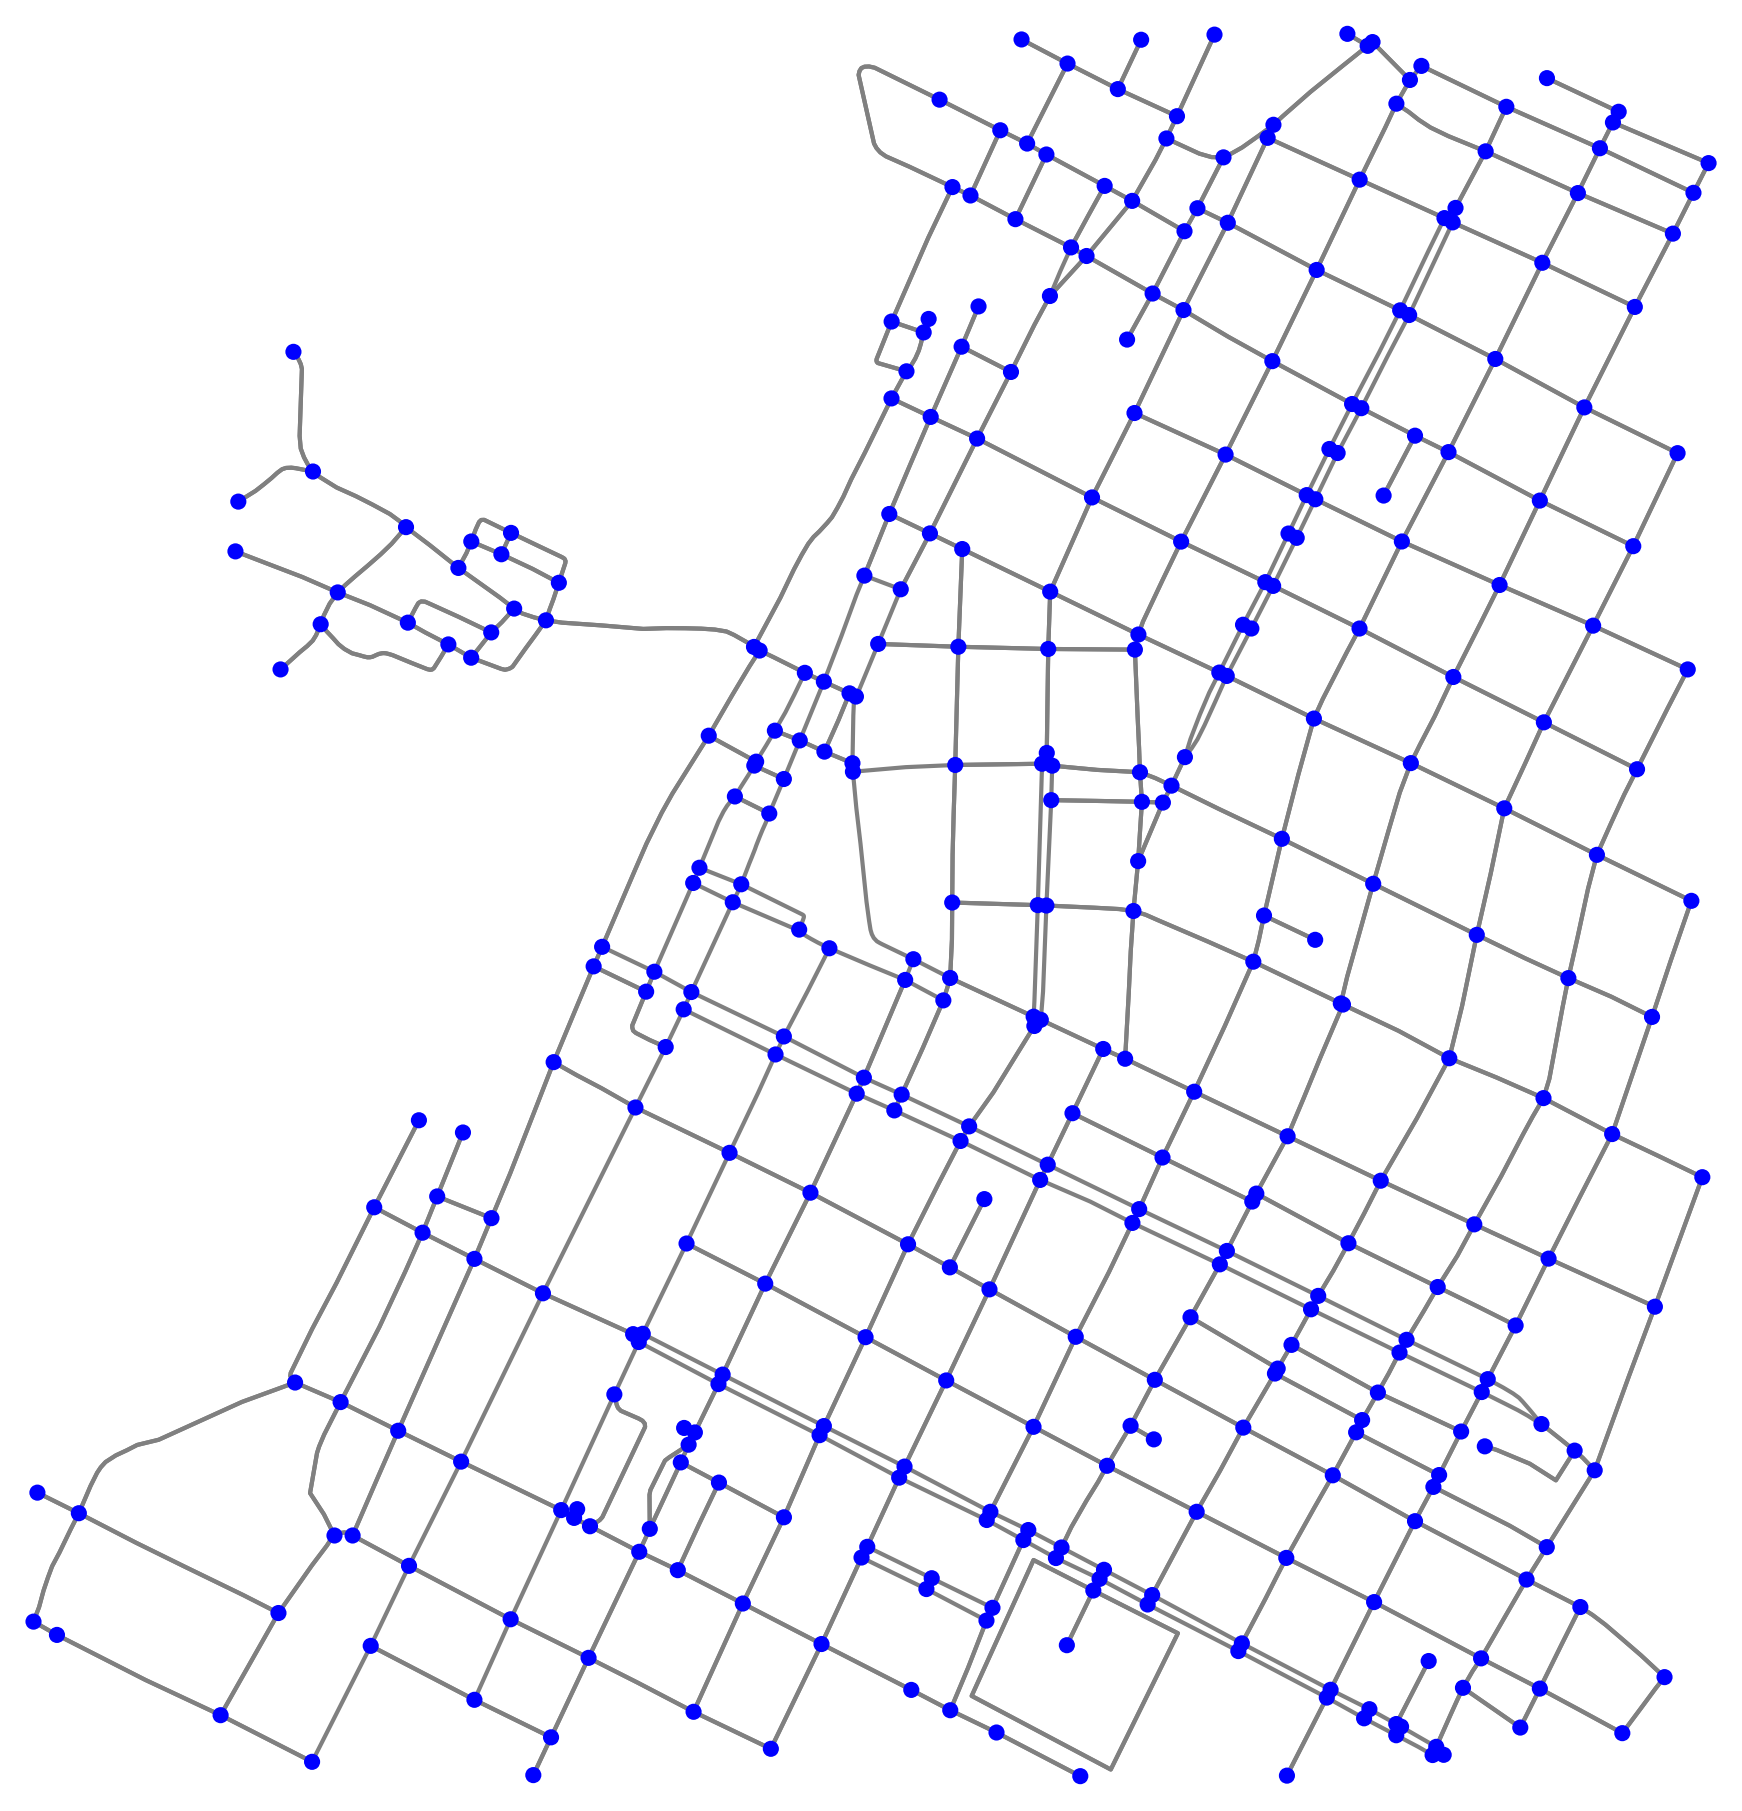
\includegraphics[width=7cm, height=6cm]{images/graph-limoeiro.png}}
	\end{minipage}
	\caption{\label{fig:graph-examples} Representation of the two cities used in the benchmark.}
\end{figure}

\subsubsection{Deterministic Benchmark}

The computational deterministic benchmark consists of 39 instances based on the real-world notifications. Table~\ref{tab:deterministic-benchmark} summarizes the key characteristics of the benchmark used in the experimental evaluation.

\begin{table}[h!]
	\centering
	\caption{Deterministic CBRP Benchmark.}
	\label{tab:deterministic-benchmark}
	\begin{tabular}{lrrrrr}
		\hline
		\multicolumn{1}{c}{Instances}                                                &
		\multicolumn{1}{c}{$|V|$}                                                    &
		\multicolumn{1}{c}{$|A|$}                                                    &
		\multicolumn{1}{c}{$|B|$}                                                    &
		\multicolumn{1}{c}{\begin{tabular}[c]{@{}c@{}}Notified\\ Cases\end{tabular}} &
		\multicolumn{1}{c}{\begin{tabular}[c]{@{}c@{}}Blocks with\\ Cases (\%)\end{tabular}}                            \\ \hline
		AS-1000-2016                                                                 & 179  & 499  & 73  & 35   & 13.70 \\
		AS-1000-2017                                                                 & 179  & 499  & 73  & 194  & 36.99 \\
		AS-1000-2018                                                                 & 179  & 499  & 73  & 196  & 36.99 \\
		AS-1000-2019                                                                 & 179  & 499  & 73  & 196  & 36.99 \\
		AS-1000-2020                                                                 & 179  & 499  & 73  & 204  & 36.99 \\
		AS-1000-2021                                                                 & 179  & 499  & 73  & 218  & 36.99 \\ \hline
		AS-2000-2016                                                                 & 253  & 684  & 88  & 26   & 9.09  \\
		AS-2000-2017                                                                 & 253  & 684  & 88  & 174  & 29.55 \\
		AS-2000-2018                                                                 & 253  & 684  & 88  & 174  & 29.55 \\
		AS-2000-2019                                                                 & 253  & 684  & 88  & 174  & 29.55 \\
		AS-2000-2020                                                                 & 253  & 684  & 88  & 181  & 29.55 \\
		AS-2000-2021                                                                 & 253  & 684  & 88  & 195  & 30.68 \\ \hline
		AS-3000-2016                                                                 & 353  & 946  & 114 & 33   & 8.77  \\
		AS-3000-2017                                                                 & 353  & 946  & 114 & 198  & 24.56 \\
		AS-3000-2018                                                                 & 353  & 946  & 114 & 198  & 24.56 \\
		AS-3000-2019                                                                 & 353  & 946  & 114 & 198  & 24.56 \\
		AS-3000-2020                                                                 & 353  & 946  & 114 & 206  & 24.56 \\
		AS-3000-2021                                                                 & 353  & 946  & 114 & 225  & 24.56 \\ \hline
		LN-1000-2015                                                                 & 372  & 1063 & 152 & 18   & 7.89  \\
		LN-1000-2016                                                                 & 372  & 1063 & 152 & 26   & 10.53 \\
		LN-1000-2017                                                                 & 372  & 1063 & 152 & 50   & 17.11 \\
		LN-1000-2018                                                                 & 372  & 1063 & 152 & 51   & 17.11 \\
		LN-1000-2019                                                                 & 372  & 1063 & 152 & 66   & 20.39 \\
		LN-1000-2020                                                                 & 372  & 1063 & 152 & 163  & 29.61 \\
		LN-1000-2021                                                                 & 372  & 1063 & 152 & 168  & 31.58 \\ \hline
		LN-2000-2015                                                                 & 980  & 2866 & 443 & 174  & 6.77  \\
		LN-2000-2016                                                                 & 980  & 2866 & 443 & 337  & 9.03  \\
		LN-2000-2017                                                                 & 980  & 2866 & 443 & 527  & 12.19 \\
		LN-2000-2018                                                                 & 980  & 2866 & 443 & 543  & 12.64 \\
		LN-2000-2019                                                                 & 980  & 2866 & 443 & 875  & 14.22 \\
		LN-2000-2020                                                                 & 980  & 2866 & 443 & 2183 & 20.99 \\
		LN-2000-2021                                                                 & 980  & 2866 & 443 & 2316 & 21.67 \\ \hline
		LN-3000-2015                                                                 & 1212 & 3497 & 517 & 169  & 5.22  \\
		LN-3000-2016                                                                 & 1212 & 3497 & 517 & 336  & 7.54  \\
		LN-3000-2017                                                                 & 1212 & 3497 & 517 & 519  & 10.83 \\
		LN-3000-2018                                                                 & 1212 & 3497 & 517 & 533  & 11.03 \\
		LN-3000-2019                                                                 & 1212 & 3497 & 517 & 860  & 12.38 \\
		LN-3000-2020                                                                 & 1212 & 3497 & 517 & 2176 & 18.96 \\
		LN-3000-2021                                                                 & 1212 & 3497 & 517 & 2315 & 19.92 \\ \hline
	\end{tabular}%
\end{table}

\subsubsection{Stochastic Benchmark}

The procedure to generate this benchmark follows the same steps as the deterministic benchmark, but with the addition of generating 50 scenarios for each instance. The first stage scenario presented in the instance is the same inputed to the \gls{mabs} presented in Chapter~\ref{chp:simulation-methodologies-and-results}. Each second stage scenario represents the aggregation, for each block, of the simulated cases generated in the 7 days after the first stage.

The stochastic benchmark consists of 36 instances based on the real-world notifications and the simulation presented in Chapter~\ref{chp:stochastic-methodologies-and-results}. Table~\ref{tab:stochastic-benchmark} summarizes the key characteristics of the benchmark used in the experimental evaluation. Each row in the table corresponds to a different instance of the stochastic benchmark. The columns correspond to the following information: the name of instance (Instance), number of nodes ($|V|$), number of arcs ($|A|$), number of blocks ($|B|$), number of scenarios ($|S|$), number of cases in the first stage scenario, number of blocks with cases in the first stage scenario, percentage of blocks with cases in the first stage scenario, number of blocks with cases in at least one scenario, number of blocks with case in at least 25\% of all scenarios, number of blocks with case in at least 50\% of all scenarios, number of blocks with case in at least 75\% of all scenarios.

The data presented in Table~\ref{tab:stochastic-benchmark} provide a detailed overview of the stochastic benchmark instances, with a focus on the distribution and persistence of notified cases across blocks and scenarios. For each municipality, three instance sizes (500, 1000, and 2000) with six variants per size, totaling 18 instances per city. All instances were evaluated using 50 stochastic scenarios to capture the inherent uncertainty in disease transmission dynamics. The instances exhibit distinct network topologies reflecting the urban structure of each municipality. Alto Santo instances range from 117 nodes and 336 arcs (size 500) to 253 nodes and 710 arcs (size 2000), covering 52 to 102 street blocks. Limoeiro do Norte presents larger networks, with instances ranging from 145 nodes, 436 arcs, and 74 blocks (size 500) to 1,008 nodes, 3,112 arcs, and 549 blocks (size 2000). 

The number of notified cases varies significantly across instances, ranging from 11 to 217 cases in Alto Santo and from 11 to 1,063 cases in Limoeiro do Norte. The spatial distribution of cases also varies considerably, with the percentage of blocks containing at least one case ranging from 18.6\% to 61.5\% in Alto Santo (mean 38.3\%) and from 9.5\% to 55.8\% in Limoeiro do Norte (mean 27.4\%), suggesting generally more concentrated spatial patterns of disease transmission in the smaller municipality.

The stochastic analysis reveals substantial uncertainty in disease spread patterns. Across all Alto Santo instances, nearly all blocks (96.2\% to 100\%) experience at least one case in at least one of the 50 scenarios. However, the persistence of disease presence decreases substantially when considering more restrictive thresholds: on average, 43.6\% of blocks present cases in at least 25\% of scenarios, 23.3\% in at least 50\% of scenarios, and only 3.2\% in at least 75\% of scenarios. 

Limoeiro do Norte exhibits even greater stochastic variability, with 87.4\% to 95.3\% of blocks experiencing cases in at least one scenario, but only 24.1\% showing cases in 25\% or more scenarios, and virtually no blocks (0.2\% on average) consistently presenting cases in 75\% or more scenarios. This pattern indicates that disease transmission in Limoeiro do Norte follows more dispersed and unpredictable spatial patterns compared to Alto Santo, highlighting the critical importance of robust optimization approaches that account for this uncertainty, as deterministic approaches based on a single scenario would fail to capture the substantial spatial and temporal variability observed in real epidemic conditions.

\begin{landscape}
\begin{table}[!ht]
    \centering
    \caption{Summary of stochastic instances including scenario-wise block coverage.}\label{tab:stochastic-benchmark}
    {\scriptsize %
        \begin{tabular}{lrrrrrrrrrrr}
            \hline
            \multicolumn{1}{c}{Instance} &
            \multicolumn{1}{c}{|V|} &
            \multicolumn{1}{c}{|A|} &
            \multicolumn{1}{c}{|B|} &
            \multicolumn{1}{c}{|S|} &
            \multicolumn{1}{c}{\begin{tabular}[c]{@{}c@{}}Cases in First\\ Stage Scenario\end{tabular}} &
            \begin{tabular}[c]{@{}l@{}}Blocks With Cases in\\ First Stage Scenario\end{tabular} &
            \begin{tabular}[c]{@{}l@{}}Blocks With Cases\\ First Stage (\%)\end{tabular} &    
            \multicolumn{1}{c}{\begin{tabular}[c]{@{}c@{}}Blocks With Cases\\ in At Least One \\ Scenario\end{tabular}} &
            \multicolumn{1}{c}{\begin{tabular}[c]{@{}c@{}}Blocks With Case \\ in At Least 25\% of \\ all Scenarios\end{tabular}} &
            \multicolumn{1}{c}{\begin{tabular}[c]{@{}c@{}}Blocks With Case \\ in At Least 50\% of \\ all Scenarios\end{tabular}} &
            \multicolumn{1}{c}{\begin{tabular}[c]{@{}c@{}}Blocks With Case \\ in At Least 75\% of \\ all Scenarios\end{tabular}} \\
            \hline
        alto-santo-500-1  & 117  & 336  & 52  & 50 & 142  & 31  & 59.6 & 52  & 28  & 14 & 2 \\
        alto-santo-500-2  & 117  & 336  & 52  & 50 & 33   & 14  & 26.9 & 51  & 28  & 19 & 3 \\
        alto-santo-500-3  & 117  & 336  & 52  & 50 & 76   & 23  & 44.2 & 52  & 30  & 14 & 2 \\
        alto-santo-500-4  & 117  & 336  & 52  & 50 & 60   & 22  & 42.3 & 52  & 27  & 19 & 3 \\
        alto-santo-500-5  & 117  & 336  & 52  & 50 & 53   & 17  & 32.7 & 51  & 29  & 19 & 0 \\
        alto-santo-500-6  & 117  & 336  & 52  & 50 & 157  & 32  & 61.5 & 52  & 28  & 19 & 2 \\ \hline
        alto-santo-1000-1 & 179  & 524  & 84  & 50 & 173  & 42  & 50.0 & 84  & 40  & 28 & 3 \\
        alto-santo-1000-2 & 179  & 524  & 84  & 50 & 38   & 18  & 21.4 & 83  & 41  & 24 & 5 \\
        alto-santo-1000-3 & 179  & 524  & 84  & 50 & 99   & 31  & 36.9 & 84  & 46  & 29 & 5 \\
        alto-santo-1000-4 & 179  & 524  & 84  & 50 & 81   & 30  & 35.7 & 82  & 40  & 22 & 4 \\
        alto-santo-1000-5 & 179  & 524  & 84  & 50 & 61   & 23  & 27.4 & 82  & 40  & 26 & 3 \\
        alto-santo-1000-6 & 179  & 524  & 84  & 50 & 195  & 43  & 51.2 & 83  & 39  & 24 & 4 \\ \hline
        alto-santo-2000-1 & 253  & 710  & 102 & 50 & 195  & 44  & 43.1 & 100 & 45  & 26 & 3 \\
        alto-santo-2000-2 & 253  & 710  & 102 & 50 & 39   & 19  & 18.6 & 101 & 50  & 29 & 1 \\
        alto-santo-2000-3 & 253  & 710  & 102 & 50 & 110  & 33  & 32.4 & 100 & 48  & 26 & 3 \\
        alto-santo-2000-4 & 253  & 710  & 102 & 50 & 81   & 30  & 29.4 & 101 & 52  & 26 & 4 \\
        alto-santo-2000-5 & 253  & 710  & 102 & 50 & 64   & 25  & 24.5 & 101 & 53  & 30 & 4 \\
        alto-santo-2000-6 & 253  & 710  & 102 & 50 & 217  & 45  & 44.1 & 101 & 43  & 26 & 4 \\ \hline
        limoeiro-500-1    & 145  & 436  & 74  & 50 & 46   & 22  & 29.7 & 67  & 8   & 0  & 0 \\
        limoeiro-500-2    & 145  & 436  & 74  & 50 & 45   & 19  & 25.7 & 67  & 7   & 0  & 0 \\
        limoeiro-500-3    & 145  & 436  & 74  & 50 & 90   & 27  & 36.5 & 71  & 6   & 0  & 0 \\
        limoeiro-500-4    & 145  & 436  & 74  & 50 & 14   & 8   & 10.8 & 66  & 4   & 0  & 0 \\
        limoeiro-500-5    & 145  & 436  & 74  & 50 & 11   & 9   & 12.2 & 68  & 5   & 0  & 0 \\
        limoeiro-500-6    & 145  & 436  & 74  & 50 & 175  & 35  & 47.3 & 69  & 9   & 0  & 0 \\ \hline
        limoeiro-1000-1   & 400  & 1260 & 231 & 50 & 134  & 67  & 29.0 & 215 & 48  & 0  & 0 \\
        limoeiro-1000-2   & 400  & 1260 & 231 & 50 & 155  & 75  & 32.5 & 219 & 38  & 0  & 0 \\
        limoeiro-1000-3   & 400  & 1260 & 231 & 50 & 256  & 100 & 43.3 & 213 & 49  & 0  & 0 \\
        limoeiro-1000-4   & 400  & 1260 & 231 & 50 & 42   & 29  & 12.6 & 214 & 48  & 0  & 0 \\
        limoeiro-1000-5   & 400  & 1260 & 231 & 50 & 26   & 22  & 9.5  & 214 & 46  & 0  & 0 \\
        limoeiro-1000-6   & 400  & 1260 & 231 & 50 & 482  & 129 & 55.8 & 212 & 55  & 0  & 0 \\ \hline
        limoeiro-2000-1   & 1008 & 3112 & 549 & 50 & 285  & 153 & 27.9 & 523 & 106 & 1  & 0 \\
        limoeiro-2000-2   & 1008 & 3112 & 549 & 50 & 353  & 167 & 30.4 & 516 & 108 & 0  & 0 \\
        limoeiro-2000-3   & 1008 & 3112 & 549 & 50 & 591  & 226 & 41.2 & 515 & 112 & 0  & 0 \\
        limoeiro-2000-4   & 1008 & 3112 & 549 & 50 & 89   & 63  & 11.5 & 523 & 101 & 1  & 0 \\
        limoeiro-2000-5   & 1008 & 3112 & 549 & 50 & 81   & 64  & 11.7 & 518 & 105 & 3  & 0 \\
        limoeiro-2000-6   & 1008 & 3112 & 549 & 50 & 1063 & 291 & 53.0 & 522 & 100 & 5  & 0 \\ \hline
        \end{tabular}
    }
    \end{table}
\end{landscape}

\section{Statistical Analysis of Results}\label{subsec:statistical-analysis}

In this work, non-parametric statistical tests were used to analyze multiple instances. The aim of using these tests is to provide a more rigorous scientific basis for the comparisons made, validating whether the difference between two or more strategies is statistically significant or not. The work of Dem\v{s}ar~\cite{demsar:2006} suggests a methodology for making such comparisons in the context of machine learning, in which various tests are used to identify the existence of \gls{ssd} among several classifiers over multiple datasets. In this section, the tests and the way to interpret their results will be briefly discussed.

For all tests, a confidence level of $95\%$ was considered, with the null hypothesis that there is no \gls{ssd} between the samples. All tests are based on \textit{ranks}, such that the approach holding \textit{rank k} is the one with the k-th best result for an instance.

The first test described is the Iman-Davenport test, used to identify the existence of \gls{ssd} among multiple approaches. Initially, it is necessary to compute the average \textit{rank} value $R_i$ for each approach. The calculation is done as follows: let $r_k^i$ be the \textit{rank} of the k-th approach for the i-th instance (with the average \textit{rank} being used in case of ties). The value $R_i$ for the i-th methodology is given by $R_i = \frac{1}{N} \cdot \sum_{k} r_k^i, \forall k \in \{1, \dots, k\}$, where $k$ is the number of approaches and $N$ the number of instances.

The value of the Iman-Davenport test is calculated according to equations \eqref{eq:x2f} and \eqref{eq:ff}.

\begin{equation}
    x^2_F = \frac{12 \cdot N}{k \cdot (k + 1)} \left[ \sum_{i} R^2_{i} - \frac{k \cdot (k+1)^2}{4} \right] \label{eq:x2f}
\end{equation}

\begin{equation}
    F_F = \frac{(N - 1) \cdot x^2_F}{N \cdot (k - 1) - x^2_F} \label{eq:ff}
\end{equation}

The value of the test calculated for $F_F$ follows the $F$ distribution, with degrees of freedom $k - 1$ and $(k - 1) \cdot (N - 1)$. Thus, the critical value can be obtained by following such a distribution. In the end, if the value $F_F$ found by the test is greater than the critical value, the null hypothesis can be rejected.

If the null hypothesis is rejected, a \textit{post-hoc} test is applied to determine which heuristics actually differ from each other. For this, the Nemenyi test is used, which calculates the critical difference and identifies groups of approaches that are statistically equivalent to each other. The results of two distinct approaches are said to be different, according to the Nemenyi test, if their average \textit{ranks} differ by at least the \gls{cd} obtained according to equation \eqref{eq:dc}.

\begin{equation}
    DC = q_{\alpha} \cdot \sqrt{\frac{l \cdot (k + 1)}{6 \cdot N}} \label{eq:dc}
\end{equation}

In equation \eqref{eq:dc}, $\alpha$ represents the confidence level, and the critical value $q_{\alpha}$ is defined according to the \textit{Studentized range} statistic divided by $\sqrt{2}$. The values of this statistic can be found in the article by De\v{m}sar \cite{demsar:2006}. Additionally, the result of the Nemenyi test can be represented graphically, as illustrated in Figure~\ref{fig:ex-nemenyi}. The horizontal axis corresponds to the average \textit{rank} values, in ascending order from left to right. Each approach is represented by a vertical line with its respective name and average \textit{rank} value just below. A horizontal line of length equivalent to the value of the CD is positioned above the main horizontal axis. Approaches with average \textit{rank} values that do not differ more than the CD are connected by a bold horizontal segment, whose length is always less than the value of the CD.

\begin{figure}[!ht] \centering
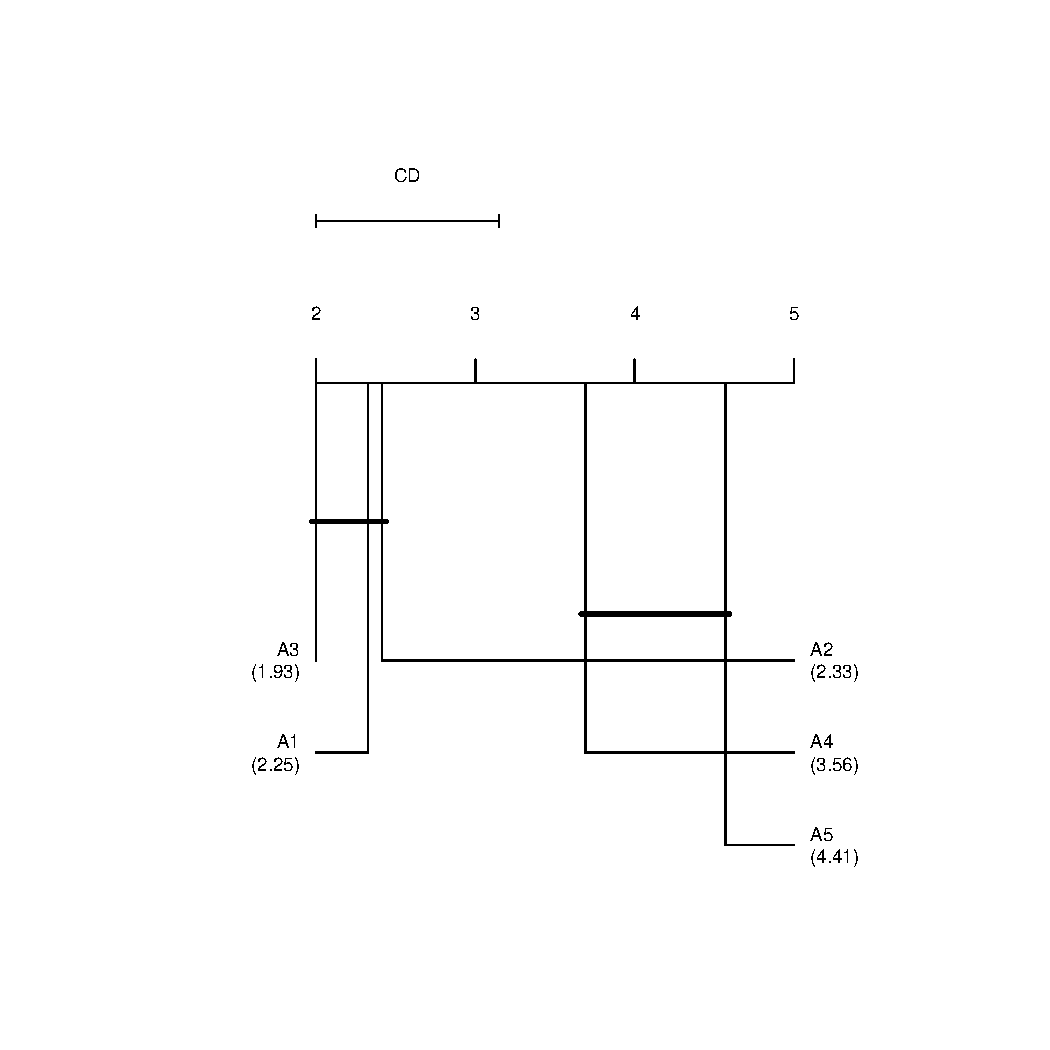
\includegraphics[scale=0.4]{images/nemenyi-example.pdf}
    \caption{Example of a graphical representation of the Nemenyi test.}
    \label{fig:ex-nemenyi}
\end{figure}

It can be observed that the fictitious approaches A3, A1, and A2 form the group with the lowest average \textit{rank} value, and consequently, are statistically equivalent to each other according to the Nemenyi test. Therefore, we may define as the best algorithm the one that presents the highest number of wins, i.e., the number of times each approach was better than the others.

Another test used in this work was the Wilcoxon test, applied when it is desired to check whether there is an SSD between the results of two methods, being more powerful than the Iman-Davenport test for this scenario. The Wilcoxon test computes the \textit{ranks} of the differences between the results of the two methods ignoring the sign, and subsequently compares the \textit{ranks} of the positive and negative differences.

To compute the Wilcoxon test, consider $d_i, i \in \{1, \dots, N\}$, the difference between the results of the two approaches for the i-th instance, and $r_{d_i}$ the \textit{rank} of the absolute value of the i-th difference (the average \textit{rank} is assigned in case of a tie). Let $R^+$ be the sum of the \textit{ranks} for the instances in which the fictitious approach A was better than B ($d_i > 0$) and $R^{-}$ the sum of the \textit{ranks} for the opposite case ($d_i < 0$). The \textit{ranks} for $d_i = 0$ are equally divided between the sums, as shown in Equation \eqref{eq:r-wilcoxon}.

\begin{equation}
    R^{+} = \sum_{d_i > 0} r_{d_i} + \frac{1}{2}\sum_{d_i = 0} \quad \quad R^{-} = \sum_{d_i < 0} r_{d_i} + \frac{1}{2}\sum_{d_i = 0} \label{eq:r-wilcoxon}
\end{equation}

Let $T = \min\{R^+, R^{-}\}$. According to Dem\v{s}ar~\cite{demsar:2006}, in cases where $N \leq 25$, the critical value for the Wilcoxon test can be found in most statistics books, such as Devore’s~\cite{devore:2011}. Once this value is calculated, the null hypothesis is rejected if the value of $T$ is less than or equal to the critical value. In cases where $N > 25$, the $z$ statistic is computed as shown in Equation~\eqref{eq:z-stat}. According to Dem\v{s}ar, considering a confidence level of $95\%$, the null hypothesis can be rejected when $z < -1.96$.

\begin{equation}
    z = \frac{T - \frac{1}{4} N(N + 1)}{\sqrt{\frac{1}{24} N(N+1)(2N + 1)}} \label{eq:z-stat}
\end{equation}
